\documentclass[12pt,a4paper]{article}

% Language setting
% Replace `english' with e.g. `spanish' to change the document language
\usepackage[english]{babel}
\usepackage{caption}
\usepackage{bigfoot} % to allow verbatim in footnote
\usepackage[numbered,framed]{matlab-prettifier}
\usepackage{longtable}

\usepackage[natbib=true,
    style=numeric,
    sorting=none]{biblatex}
\addbibresource{sample.bib}



\let\ph\mlplaceholder % shorter macro
\lstMakeShortInline"

\lstset{
  style              = Matlab-editor,
  basicstyle         = \footnotesize  \mlttfamily,
  escapechar         = ",
  mlshowsectionrules = true,
  numberstyle = \scriptsize \color{gray}\mlttfamily,
}

\captionsetup{format=plain, font={footnotesize}}
%https://tex.stackexchange.com/questions/75116/what-can-i-use-to-typeset-matlab-code-in-my-document

% Set page size and margins
% Replace `letterpaper' with`a4paper' for UK/EU standard size
\usepackage[a4paper,top=3cm,bottom=3cm,left=3cm,right=3cm,marginparwidth=1.75cm]{geometry}
\usepackage{fourier}

% Useful packages
\usepackage{amsmath}
\usepackage{graphicx}
\usepackage[colorlinks=true, allcolors=blue]{hyperref}
\usepackage{amssymb}
\usepackage{amsthm}



\newcommand{\N}{\mathbb{N}}
\newcommand{\Z}{\mathbb{Z}}
\newcommand{\Q}{\mathbb{Q}}
\newcommand{\C}{\mathbb{C}}
\newcommand{\D}{\mathbb{D}}
\newcommand{\R}{\mathbb{R}}
\newcommand{\F}{\mathbb{F}}
\newcommand{\T}{\mathcal{T}}
\newcommand{\U}{\mathcal{U}}
\newcommand{\LL}{\mathcal{L}}
\newcommand{\Holder}{H$\ddot{\text{o}}$lder}
\newcommand{\Hi}{\mathcal{H}}
\newcommand{\Res}{\text{Res}}
\newcommand{\rt}{\rho_\theta}

\theoremstyle{definition}
\newtheorem{thm}{Theorem}
\newtheorem{defn}{Definition}
\newtheorem{cor}[thm]{Corollary}
\newtheorem{lemma}[thm]{Lemma}
\newtheorem*{rmk}{Remark}
\newtheorem*{joke}{Joke}
\newtheorem{ex}{Example}[subsection]
\newtheorem*{soln}{Solution}
\newtheorem{prop}[thm]{Proposition}


\title{Numerical Methods of Stochastic Differential Equation and }
\author{Yihuan Dong}

\begin{document}
\maketitle


\section{Introduction}
As a first-year VISP student with a research interest in financial mathematics, I am highly motivated to explore the potential of mathematical tools in solving financial problems. One of the most important tools in this field is the stochastic differential equation (SDE), which is widely used in analyzing portfolio and risky assets. With the aim of preparing myself for a Ph.D. in this area, I plan to undertake a project that focuses on numerical methods for SDE and their applications in finance.

The project will be divided into several sections, each building on the previous one to
provide a detailed understanding of the topic.

In this paper, we explore numerical methods for Stochastic Differential Equations (SDEs) with a focus on the Euler-Maruyama and Milstein methods. To begin, we introduce the Wiener process, which forms the foundation of SDEs, and the discrete Wiener process, which is widely used in computational methods. We then define the Stochastic Integral and Stochastic Differential Equations, and present a computational method based on the partition of integrals and ODE.

In the next section, we introduce the Euler-Maruyama method, which is derived using Ito-Taylor Expansion and Ito Lemma. We then compute the error of this method in MATLAB and discuss its convergence, including strong and weak convergence. We test the convergence using two methods: comparing the slope of the plot and computing the real order $q$ and comparing it with the true order.

The fourth section focuses on the Milstein method, which is more precise than the Euler-Maruyama method since it includes two-order terms in the Ito-Taylor expansion. We compare the error between the two methods to provide a more intuitive illustration of their differences.

In the fifth section, we discuss the stability of the Euler-Maruyama method. We address two categories of stability, mean-square stability and asymptotic stability, and explore the relationship between coefficients and stability, including SDE stability and stability under the Euler-Maruyama method.

In the final section, we presented the definition and generation techniques of quasi-random numbers, also known as low-discrepancy numbers. This new class of random numbers offers the advantage of reducing the error between the numerical method solution (we take the Euler-Maruyama method as an example) and the true solution. Furthermore, to eliminate the reliance on random numbers in the true solution, we introduced the use of European call options in this section.

This project references papers primarily based on \cite{higham._2001} and \cite{sauer}, and other sources for obtaining formulas and algorithms. All files, including MATLAB \verb|.m| projects, are accessible through the provided link.
\section{Wiener Process}

To study asset pricing in financial mathematics, we model asset prices as continuous time stochastic process, and analyse it by \textbf{diffusion process} and \textbf{stochastic differential equations(SDE)}. To introduce the concept of diffusion, we say that a stochastic process $X$ is as diffusion if its local dynamics can be approximated by a stochastic difference equation of the following type(\cite{bjork}, P43, 4.1):\begin{equation}
    \label{eq-diffusion}X_{t+\Delta t}-X_t=\mu(t,X_t)\Delta t+\sigma(t,X_t)Z_t,
\end{equation}
where $Z_t$ is a normally distributed disturbance term and it is independent of what was happening in time $t$, $\mu(t,X_t)$ is a locally deterministic velocity (called the \text{drift} term of the process) and $\sigma(t,X_t)$ is the amplifying factor of a Gaussian disturbance term (called the \textbf{diffusion} term).

Then we introduce the concept of Wiener process, which is also called Brownian Motion.

\begin{defn}\label{defn1}
    A stochastic process $W$ is called a \textbf{Wiener process} if the following conditions hold.

    (i) $W(0)=0.$

    (ii) The process $W$ has independent increments, i.e. if $r<s\le t<u$, then $W(u)-W(t)$ and $W(s)-W(r)$ are independent random variables. 

    (iii) For $s<t$ the random variable $W(t)-W(s)$ has the Gaussian distribution $N(0,t-s)$ (Or $W(t)-W(s)\sim\sqrt{t-s}N(0,1)$\cite{higham._2001}).

    (iv) $W$ has contiuous trajectories.
\end{defn}

The Wiener process is named after American mathematician Norbert Wiener who investigated the mathematical properties of the one-dimensional Brownian motion. 

The standard Wiener process is studied in continuous time, but in numerical analysis, we consider discretized form of it, where $W(t)$ is specified at discrete $t$ values and we set $\delta t=T/N$ for some positive integer $N$ and $W_j$ denote $W(t_j)$ with $t_j=j\delta t$\ ($j=1,\dots, n$). \ref{defn1}.(i) says that $W_0=0$ with probability 1 and \ref{defn1}.(ii) and (iii) shows that \begin{equation}
    \label{2.1}
    W_j=W_{j-1}+dW_j,\quad j=1,2,\dots,N,
\end{equation}
where each $dW_j$ is independent of the form $\sqrt{\delta t} N(0,1)$.\cite{higham._2001}

We produce the discreted Wiener process in MATLAB by command \verb|randn|. However, the numbers produced by \verb|randn| is not truly random numbers because computers are deterministic devices — a computer's behavior is entirely predictable, by design\cite{computer}. We can improve the accuracy by using \textbf{quasi-random number} instead\cite{sauer}\cite{matlab-quasi}, where we will discuss it in later. 

Now we use command \verb|randn| to produce a discrete Weiner process (\verb|wpro.m|). 

\lstinputlisting[caption = {Generate a discrete Weiner process with 200 points}, captionpos=b, label={lst1}]{matlab/wpro.m}

And we draw the path of Listing \ref{lst1} as follow:
\begin{figure}[htbp]
\centering
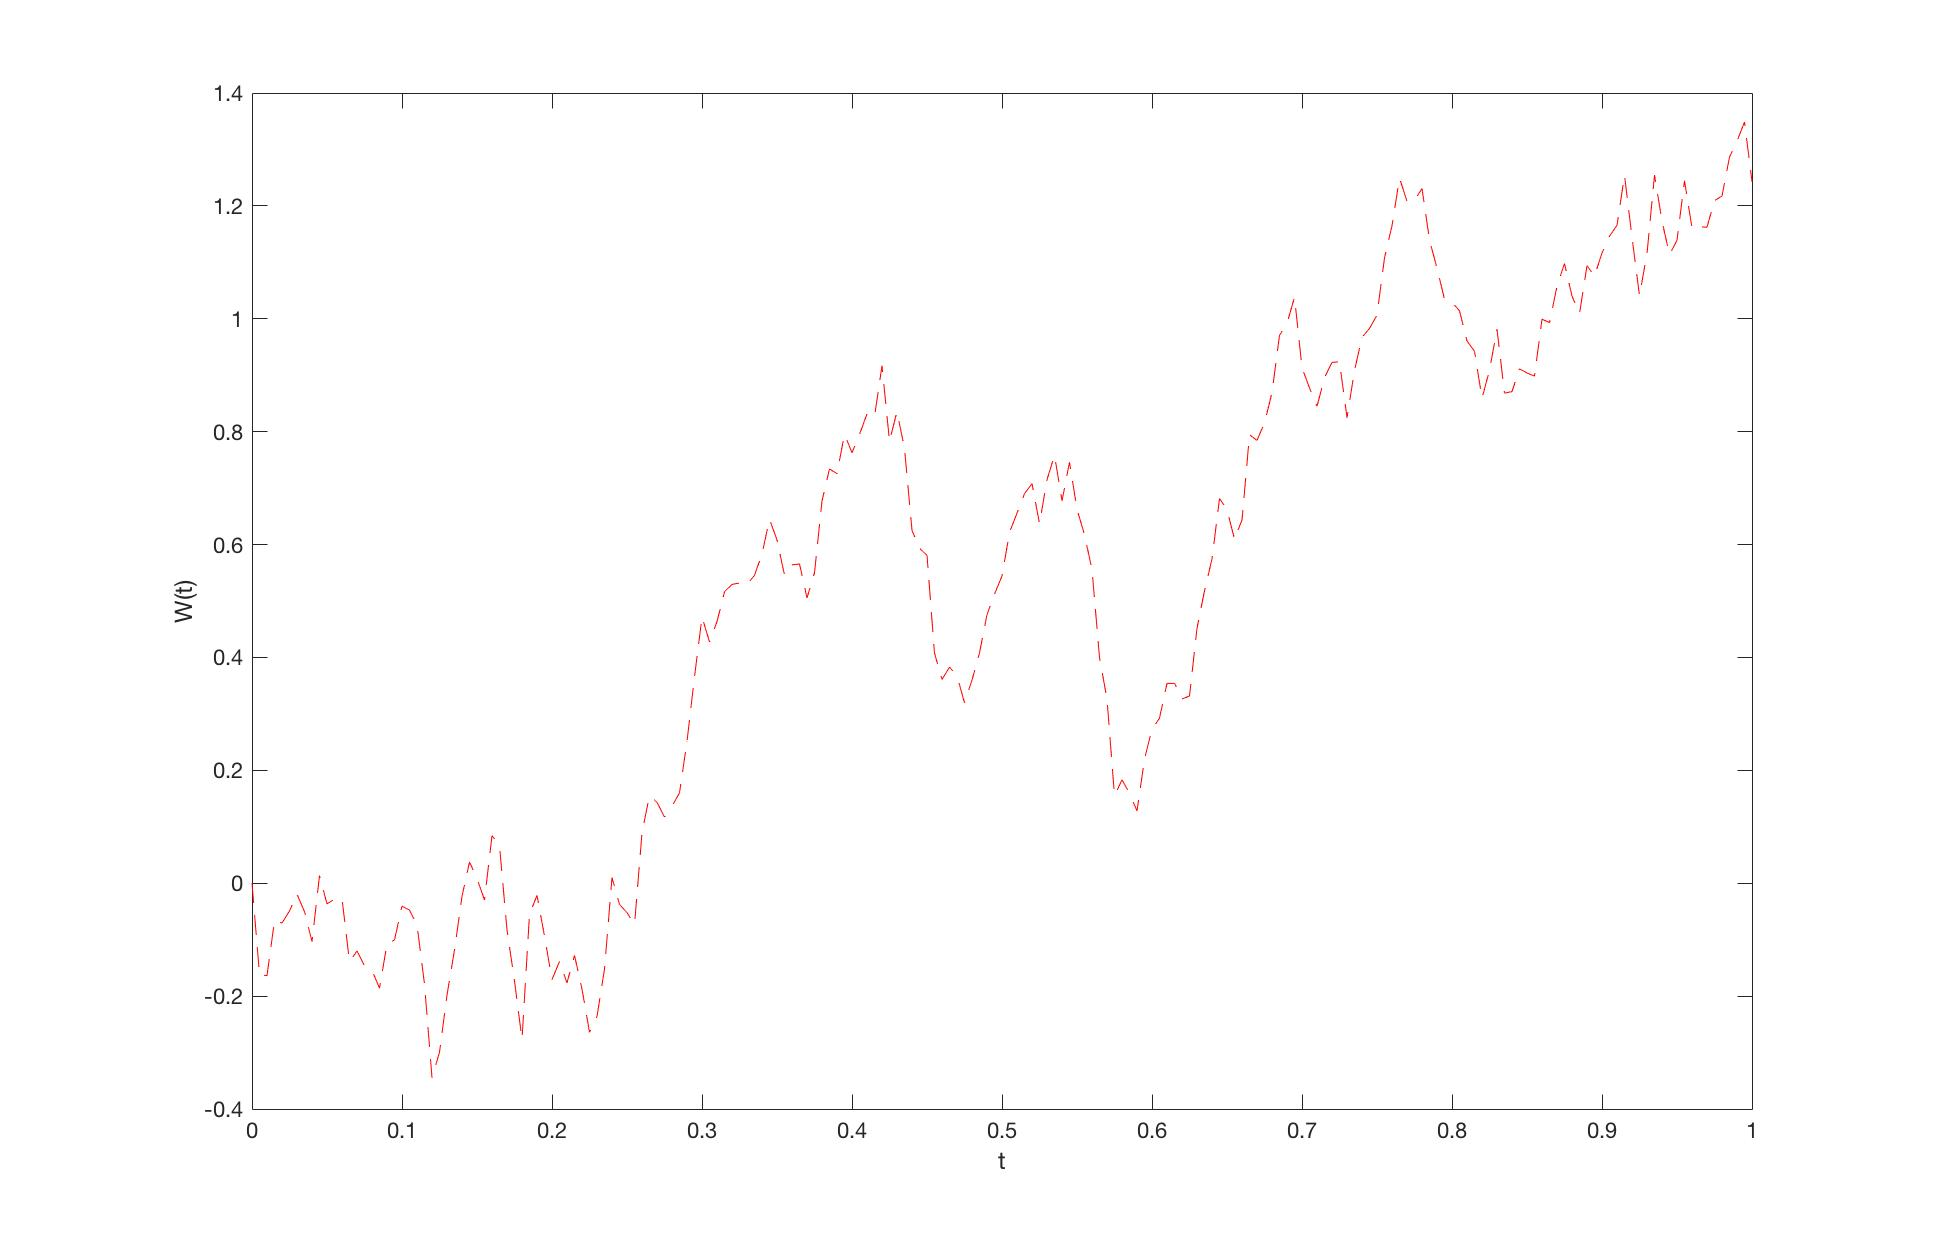
\includegraphics[width=0.9\textwidth]{fig/fig1.jpg}
\caption{\label{fig1}A discrete Wiener process}
\end{figure}



\section{Stochastic Integrals and Stochastic Differential Equation}

A typical diffusion process in finance is usually modeled as a differential equation, which can be expressed as follows\cite{sauer}:
\begin{equation}
    \label{SDE1}
    dX=a(t,X)dt+b(t,X)dW_t,
\end{equation}
where combines deterministic (or drift) terms and stochastic (or diffusion) terms. The latter term $dW_t$ represents a Wiener process. This category of SDE is often used in financial mathematics, often called \textbf{Black-Scholes Equation}, which is written as \cite{sauer}:
\begin{equation}
    \label{B-S} dX=\mu X\, dt+\sigma X\, dW_t,\quad X(t_0)=X_0.
\end{equation}
where $\mu$ and $\sigma$ are constants. The solution of equation (\ref{B-S}) coule be written as:\begin{equation}
    \label{B-Ss} X(t)=X_0e^{(\mu-\frac{1}{2}\sigma^2)t+\sigma W_t}.
\end{equation}

Now we take (\ref{SDE1}) as integral eqaution:
\begin{equation}
    \label{SDE2}
    X(t)=X(0)+\int_{t_0}^t a(s,X(s))\,ds+\int_{t_0}^t b(s,X(s))\, dW_s.
\end{equation}

By the definition of Riemann integral, the former integral could be written by:$$
\int_{t_0}^t a(s,X(s))\,ds=\lim_{n\to\infty}\sum_{j=1}^{n}a(t_j', X(t_j'))\Delta t_j,
$$
where we set $0=t_0<t_1<\dots<t_{n-1}<t_n=t$, $\Delta t_j = t_j-t_{j-1}$, and $t_{j-1}\le t_j'\le t_j$. The latter integral is Riemann-Stieljes integral, which could be represented by \cite{Bullock}:
$$
\int_{t_0}^t b(s,X(s))\, dW_s = \lim_{n\to \infty} \sum_{j=1}^{n}b(t_j', X(t_j'))\Delta W(t_j),
$$
where we set $\Delta W(t_j)=W(t_{j+1})-W(t_j)$. Therefore, we can use the sum of series to approximate these integrals. Based on the comparison results presented in \cite{higham._2001}, P531, we select the Ito integral as our approximation method. In other words, we set the 'left-hand' point $t_j'=t_{j-1}$. Those integrals could be written as:\begin{equation}
\label{3.1}
    \int_{t_0}^t a(s,X(s))\,ds\approx  \sum_{j=1}^{N}a(t_{j-1}, X(t_{j-1}))(t_{j}-t_{j-1}),
\end{equation} 
\begin{equation}
\label{3.2}
    \int_{t_0}^t b(s,X(s))\, dW_s \approx \sum_{j=1}^{N}b(t_{j-1}, X(t_{j-1}))(W(t_{j})-W(t_{j-1}))
\end{equation} 
for large $N$.


\section{Euler-Maruyama(EM) Method}
\subsection{Ito-Taylor Expansion}
To obtain the numerical methods of SDE, we firstly introduce Ito-Taylor expansion for the stochastic case (\cite{bayram}, 3.1). Consider the SDE:\begin{equation}
    \label{333}
    dX(t) = f(X(t))\, dt + g(X(t))\, dW(t),\quad X(0)=X_0, \quad 0\le t\le T.
\end{equation}
where $f$ and $g$ satisfy a linear growth bound and are smooth functions.

Assume $F\in C^2(\R)$, from Ito lemma we have (\cite{bjork}, Th4.11):\begin{equation}
    \label{itolemma}dF[X(t)]=\left\{f[X(t)]\frac{\partial F[X(t)]}{\partial X}+\frac{1}{2}g^2[X(t)]\frac{\partial^2F[X(t)]}{\partial X^2} \right\}dt+g[X(t)]\frac{\partial F[X(t)]}{\partial X} dW(t)
\end{equation}

We define operators as follow:
\begin{equation}
    \label{L0}L^0:=f[X(t)]\frac{\partial }{\partial X}+\frac{1}{2}g^2[X(t)]\frac{\partial^2}{\partial X^2},
\end{equation}
\begin{equation}
    \label{L1}L^1:=g[X(t)]\frac{\partial }{\partial X} .
\end{equation}
Then we rewrite the equation (\ref{itolemma}) as:
\begin{equation}
    \label{ito2}
    dF[X(t)]=L^0 F[X(t)]\, dt+L^1F[X(t)]\, dW(t)
\end{equation}
Take integral form of it:
\begin{equation}
    \label{ito3}
    F[X(t)]=F[X(t_0)]+\int_{t_0}^t L^0 F[X(s)]\,ds+\int_{t_0}^t L^1 F[X(s)]\, dW(s).
\end{equation}

Take $F(x)=x, F(x)=f(x)$ and $F(x)=g(x)$ respectively, we have:
\begin{equation}
    \label{eq9}X(t)=X(t_0)+\int_{t_0}^t f[X(s)]\,ds+\int_{t_0}^t g[x(s)]\, dW(s),
\end{equation}

\begin{equation}
    \label{eq10}f[X(t)]=f[X(t_0)]+\int_{t_0}^t L^0 f[X(s)]\,ds+\int_{t_0}^t L^1 f[x(s)]\, dW(s),
\end{equation}

\begin{equation}
    \label{eq11}g[X(t)]=g[X(t_0)]+\int_{t_0}^t L^0 g[X(s)]\,ds+\int_{t_0}^t L^1 g[x(s)]\, dW(s),
\end{equation}
Put (\ref{eq10}) and (\ref{eq11}) into (\ref{eq9}), we have, \begin{align}
    X(t)=X(t_0) &+\int_{t_0}^t\left(f[X(t_0)]+\int_{t_0}^{s_1} L^0 f[X(s_2)]\,ds+\int_{t_0}^{s_1} L^1 f[x(s_2)]\, dW(s_2) \right) ds_1 \nonumber \\
    &+ \int_{t_0}^t\left(g[X(t_0)]+\int_{t_0}^{s_1} L^0 g[X(s_2)]\,ds_2+\int_{t_0}^{s_1} L^1 g[x(s_2)]\, dW(s_2) \right) dW(s_1).
\end{align}

Thus we have:
\begin{equation}
    \label{eq13}X(t)=X(t_0)+f[X(t_0)]\cdot (t-t_0)+g[X(t_0)](W(t)-W(t_0))+\mathcal{R}
\end{equation}
where \begin{align}
    \mathcal{R}&= \int_{t_0}^t\int_{t_0}^{s_1} L^0f[X(s_2)]\, ds_2ds_1+ \int_{t_0}^t\int_{t_0}^{s_1} L^1f[X(s_2)]\, dW(s_2)ds_1 \nonumber \\
    &\quad +\int_{t_0}^t\int_{t_0}^{s_1} L^0g[X(s_2)]\, ds_2dW(s_1)+ \int_{t_0}^t\int_{t_0}^{s_1} L^1g[X(s_2)]\, dW(s_2)dW(s_1).
\end{align}

Equation (\ref{eq13}) contains main terms and remaining term $\mathcal{R}$, if we ignore the remaining term $\mathcal{R}$, we could obtain Euler-Maruyama method. If we make futther expansion on $\mathcal{R}$ (see \cite{bayram}, (15)-(18)), and by using Ito lemma again, we have \begin{align}
    X(t)& = X(t_0)+f[X(t_0)]\cdot t+g[X(t_0)](W(t)-W(t_0))\nonumber \\
    &\quad + g[X(t_0)]g'[X(t_0)]\left\{ \frac{1}{2}[W(t)-W(t_0)]^2 -\frac{1}{2}t\right\}+\tilde{\mathcal{R}} \label{eq19}
\end{align} 
where $\tilde{\mathcal{R}}$ is the remaining term. From equation (\ref{eq19}), we could obtain Milstein method.

\subsection{EM Methods}
The Euler-Maruyama method is a numerical method for solving a SDE. It is named after a famous mathematician Euler and Japanese mathematician Gisiro Maruyama. Maruyama, who immediately recognized the importance of Kiyosi Ito's work on SDE, published a series of papers on stochastic differential equations and Markov processes, particularly for his 1955 study of the convergence properties of the finite-difference approximations for the numerical solution of stochastic differential equations. 

Consider SDE (\ref{333}), and by using Ito-Taylor expansion in form (\ref{eq13}), we obtain EM methods as follows:
\begin{equation}
    \label{emmethods}X(t_{i+1})=X(t_i)+f(X(t_i))\Delta t_i + g(X(t_i))\Delta W_i
\end{equation}
for $i=0,1,2,\dots, N-1$ with the initial value $X(0)=X_0$, where $\Delta t_i=t_{i+1}-t_i$ and $\Delta W(t_i)=W(t_{i+1})-W(t_i)$.

We apply this method in Black-Scholes Equation (\ref{B-S}), the corresponding EM equations have the form as:\begin{equation}\label{emeq1}
    X(t_{i+1})=X(t_i)+\mu X(t_i)\Delta t_i+\sigma X(t_i) \Delta W(t_i),\quad X(0)=X_0.
\end{equation}
For a serie of a stock, we could use the method of maximum estimate(ME) from \cite{Lo}.eqn(31), which is \begin{equation}
    \label{esti}\hat{\mu}= \frac{1}{T}\sum_{k=1}^N\left( \frac{X_k}{X_{k-1}}-1\right),\quad \hat{\sigma}^2=\sum_{k=1}^N\left( \frac{X_k}{X_{k-1}}-1-\hat{\mu}h\right)^2
\end{equation} 
where $h=\Delta t$ (the time intervel). Except ME, we can also apply non-parametric parameter estimation methods\cite{mustafa} to estimate $\mu$ and $\sigma$. In this section, we apply the opening stock prices of Apple Inc. (AAPL) from 05/02/2022 to 04/28/2023 for 250 trading days (\cite{AAPL}, see the csv file \verb|AAPL.csv| ). We use MATLAB to plot the stock and estimate the drift coefficient $\mu$ and diffusion coefficient $\sigma$ as follow:

\lstinputlisting[caption = ME eatimate of AAPL, captionpos=b, label={lst2}]{matlab/me1.m}
\begin{figure}[htbp]
\centering
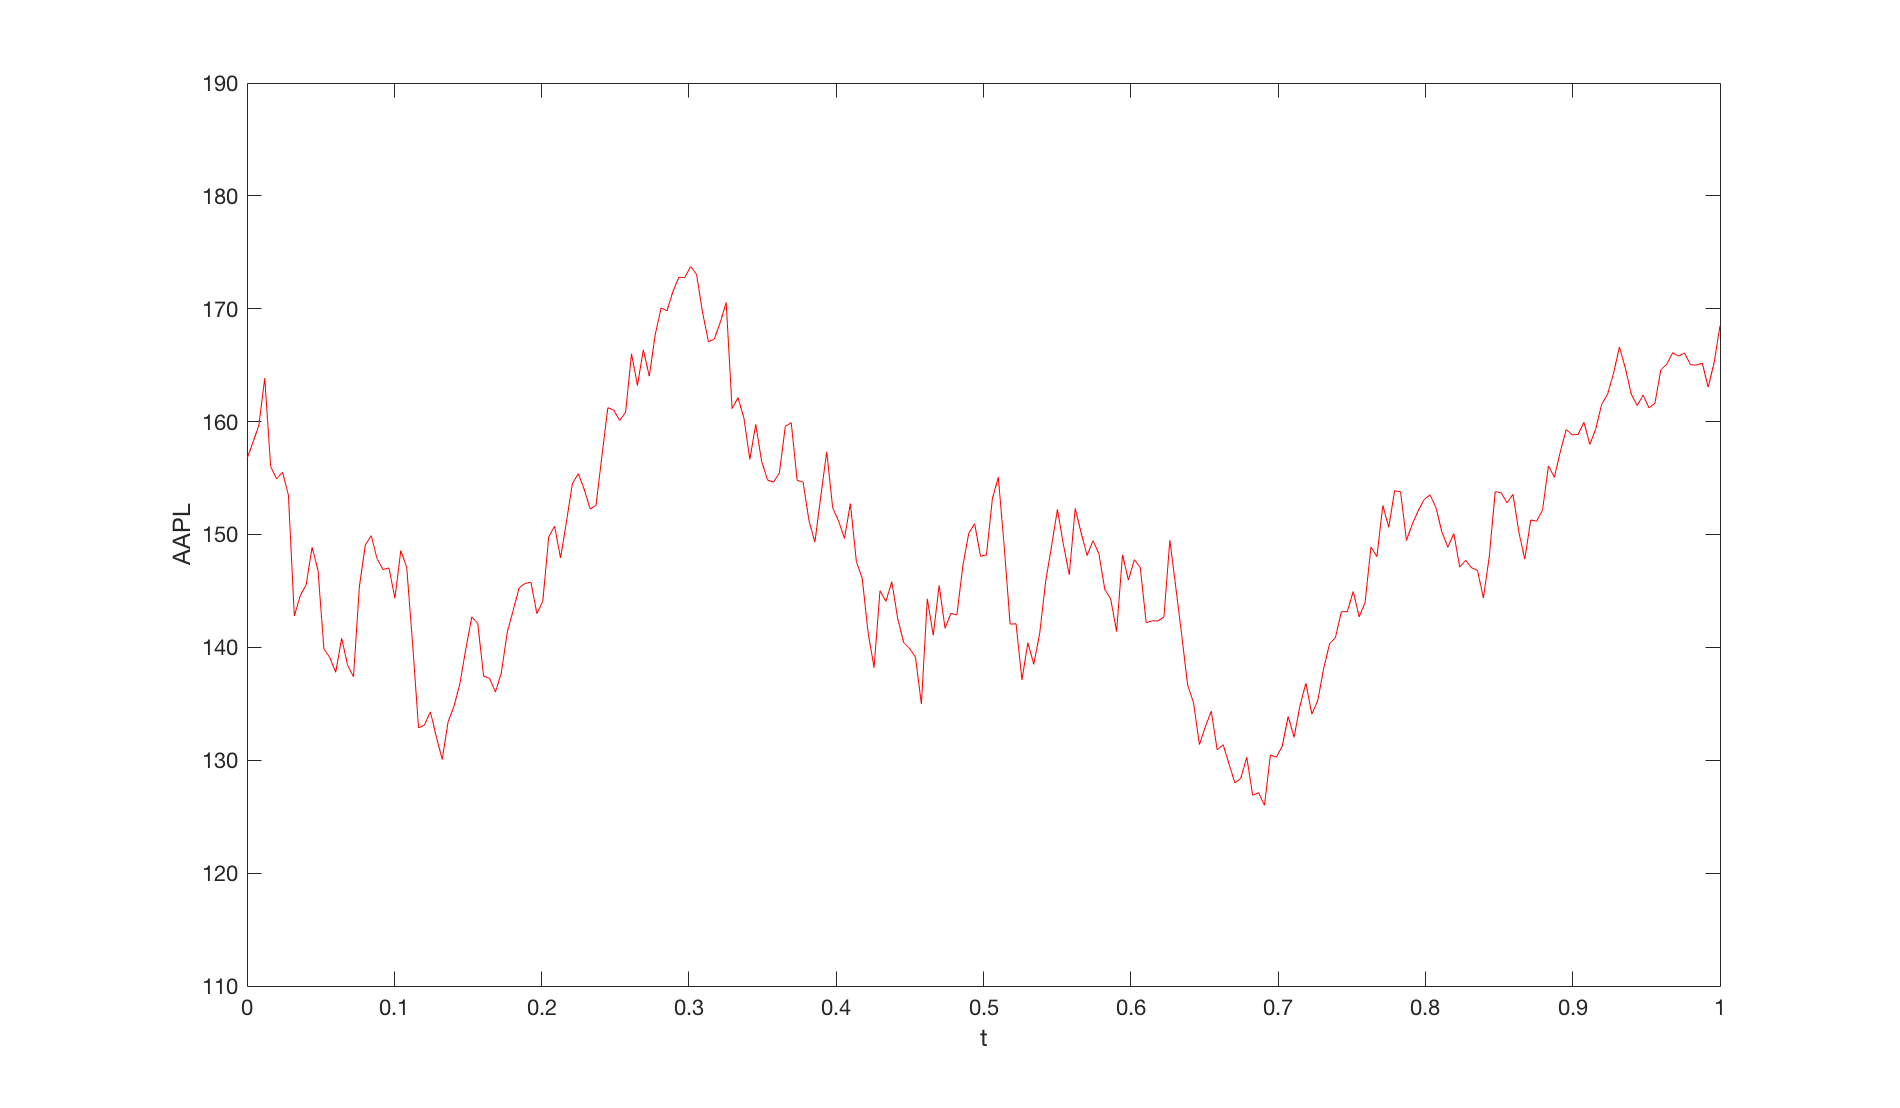
\includegraphics[width=0.8\textwidth]{fig/AAPL.png}
\caption{\label{AAPLplot}The opening price of AAPL in the stock market from 05/02/2022 to 04/28/2023}
\end{figure}

From Listing \ref{lst2} (\verb|me1.m|), we have the estimate $\hat{\mu}=0.1244$ and $\hat{\sigma}=0.1038$. Thus can write equation (\ref{emeq1}) as:\begin{equation}\label{emeq2}
    X(t_{i+1})=X(t_i)+0.1244 X(t_i)\Delta t_i+0.1038 X(t_i) \Delta W(t_i),\quad X(0)=156.71.
\end{equation}




From (\ref{B-Ss}), the true solution of $X_{true}(t)$ is:
\begin{equation}
    \label{trueAAPL} X_{true}(t)= 156.71 e^{0.1190t+0.1038W_t}.
\end{equation}

We then utilize the EM method to solve this equation and compare our results with the true solution in MATLAB. Thanks to Listing 5 in \cite{higham._2001} provides us with the necessary code to solve our equation using the EM method. We just need to do is input our coefficients and initial values. The code for the EM method to solve equation (\ref{emeq2}) is as follows:

\lstinputlisting[caption = EM-method , captionpos=b, label={lst3}]{matlab/em1.m}
\begin{figure}[htbp]
\centering
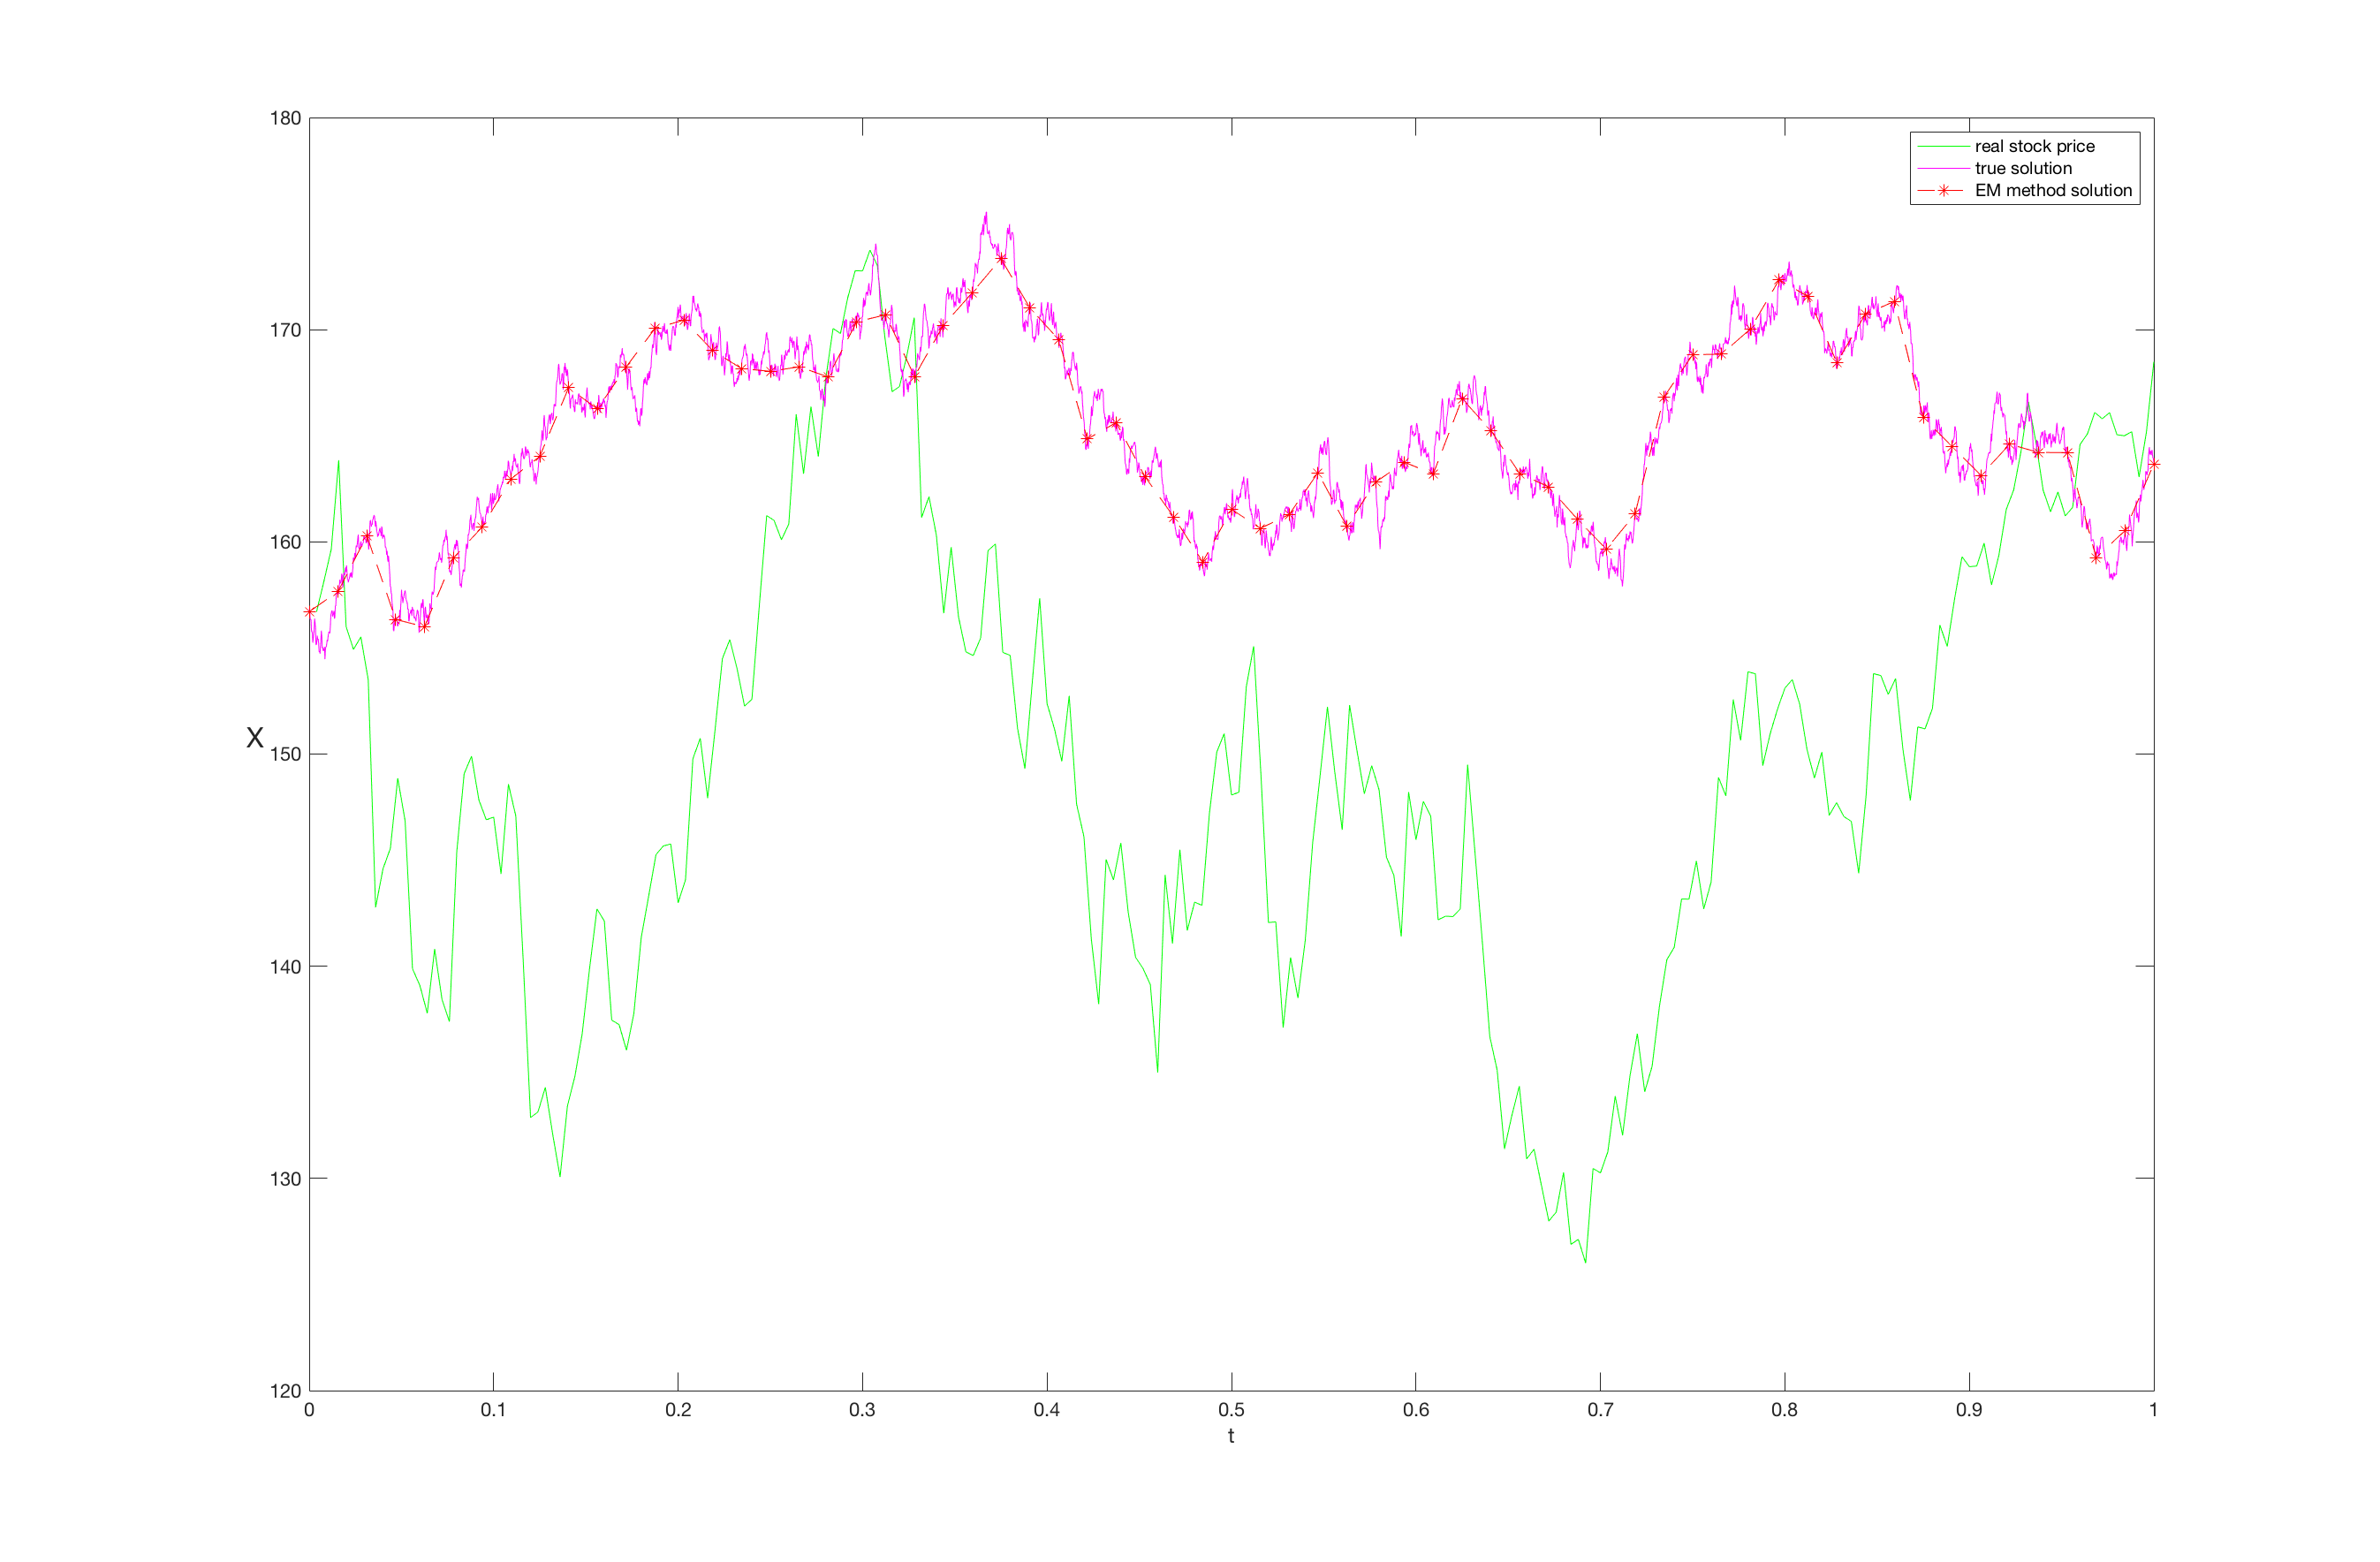
\includegraphics[width=0.8\textwidth]{fig/fig3.png}
\caption{\label{em1plot}Real stock price, true solution and EM solution}
\end{figure}

In this program (Listing \ref{lst3}, see in \verb|em1.m|) we take the discrete interval as $\Delta t = 2^{-6}$. The plots of true solution and EM method solution is shown in Fig \ref{em1plot}. Define the absolute error between true solution and EM method solution in time $T=1$ as:\begin{equation}
    \label{emerreq}\varepsilon_{EM}=|X_{true}(T)-X(T)|
\end{equation}
In  \verb|em1.m|, we use \verb|emerr| denote it. When $\Delta t = 2^{-6}$, \verb|emerr=0.0645|. If we take $\Delta t$ smaller as $2^{-N}$, $N=7,8,9,10,11$, corresponding \verb|emerr| are as follow:
\begin{longtable}[c]{lllllll}
\hline
\textbf{$N$} & \textbf{6} & \textbf{7} & \textbf{8} & \textbf{9} & \textbf{10}&\textbf{11} \\ \hline
\endfirsthead
%
\endhead
%
\verb|emerr| &  0.0645 &   0.0666  &  0.0719  &  0.1034 &   0.0842 &   0.0489\\ \hline
\caption{error of different length of interval ($2^{-N}$)}
\label{tab:my-table}\\
\end{longtable}


\subsection{Convergence of EM method}
After introducing the EM method for solving an SDE, we must consider a significant issue: Does the EM solution converge to the true solution for every $t\in [0,T]$? And as $\Delta t \to 0$, does the EM method solution converge closely to the true solution?

We first consider strong convergence, a discrete-time approcimation is called \textbf{strongly converge} at time $T$ if \cite{sauer}:$$
\lim_{\Delta t\to 0}\mathbb{E}|X_{true}(T)-X(T)|=0,
$$ 
We define the order of the strong convergence as(\cite{higham._2001},eqn 5.1):
\begin{equation}
    \label{strcon} \mathbb{E}|X_{true}(\tau)-X(\tau)|\le C\Delta t^\gamma
\end{equation}
for some constant $C$(not related to $t\in [0,T]$) and every $\tau = n\Delta t$ ($n$ is the $n$-th interval), provided $\Delta t$ is sufficiently small. We denote $\gamma$ as the order of such strong convergence. In numerical analysis, we focus on the end point $t=T(=1)$ and from \cite{higham._2001}, we know the order of strong convergence of linear SDE is $\frac{1}{2}$. Now we test this order in our equation (\ref{emeq2}) and (\ref{trueAAPL}). We denote the error as\begin{equation}
    \label{emerr}\varepsilon^{str}_{\Delta t}:=\mathbb{E}|X_{true}(T)-X(T)|
\end{equation}


First, we evaluate 10,000 sample paths for $N=2^6,2^7,2^8,2^9,2^{10}$ and plot the first 20 paths on a graph. Next, we calculate the mean of the 10,000 values and determine its error. We perform these steps in MATLAB as follows(see in \verb|strongcon_em.m|):
\lstinputlisting[caption = {Ploting paths (Fig.\ref{fig4}) and comparing with real order 0.5}, captionpos=b, label={lst4}]{matlab/strongcon_em.m}

\begin{figure}[htbp]
\centering
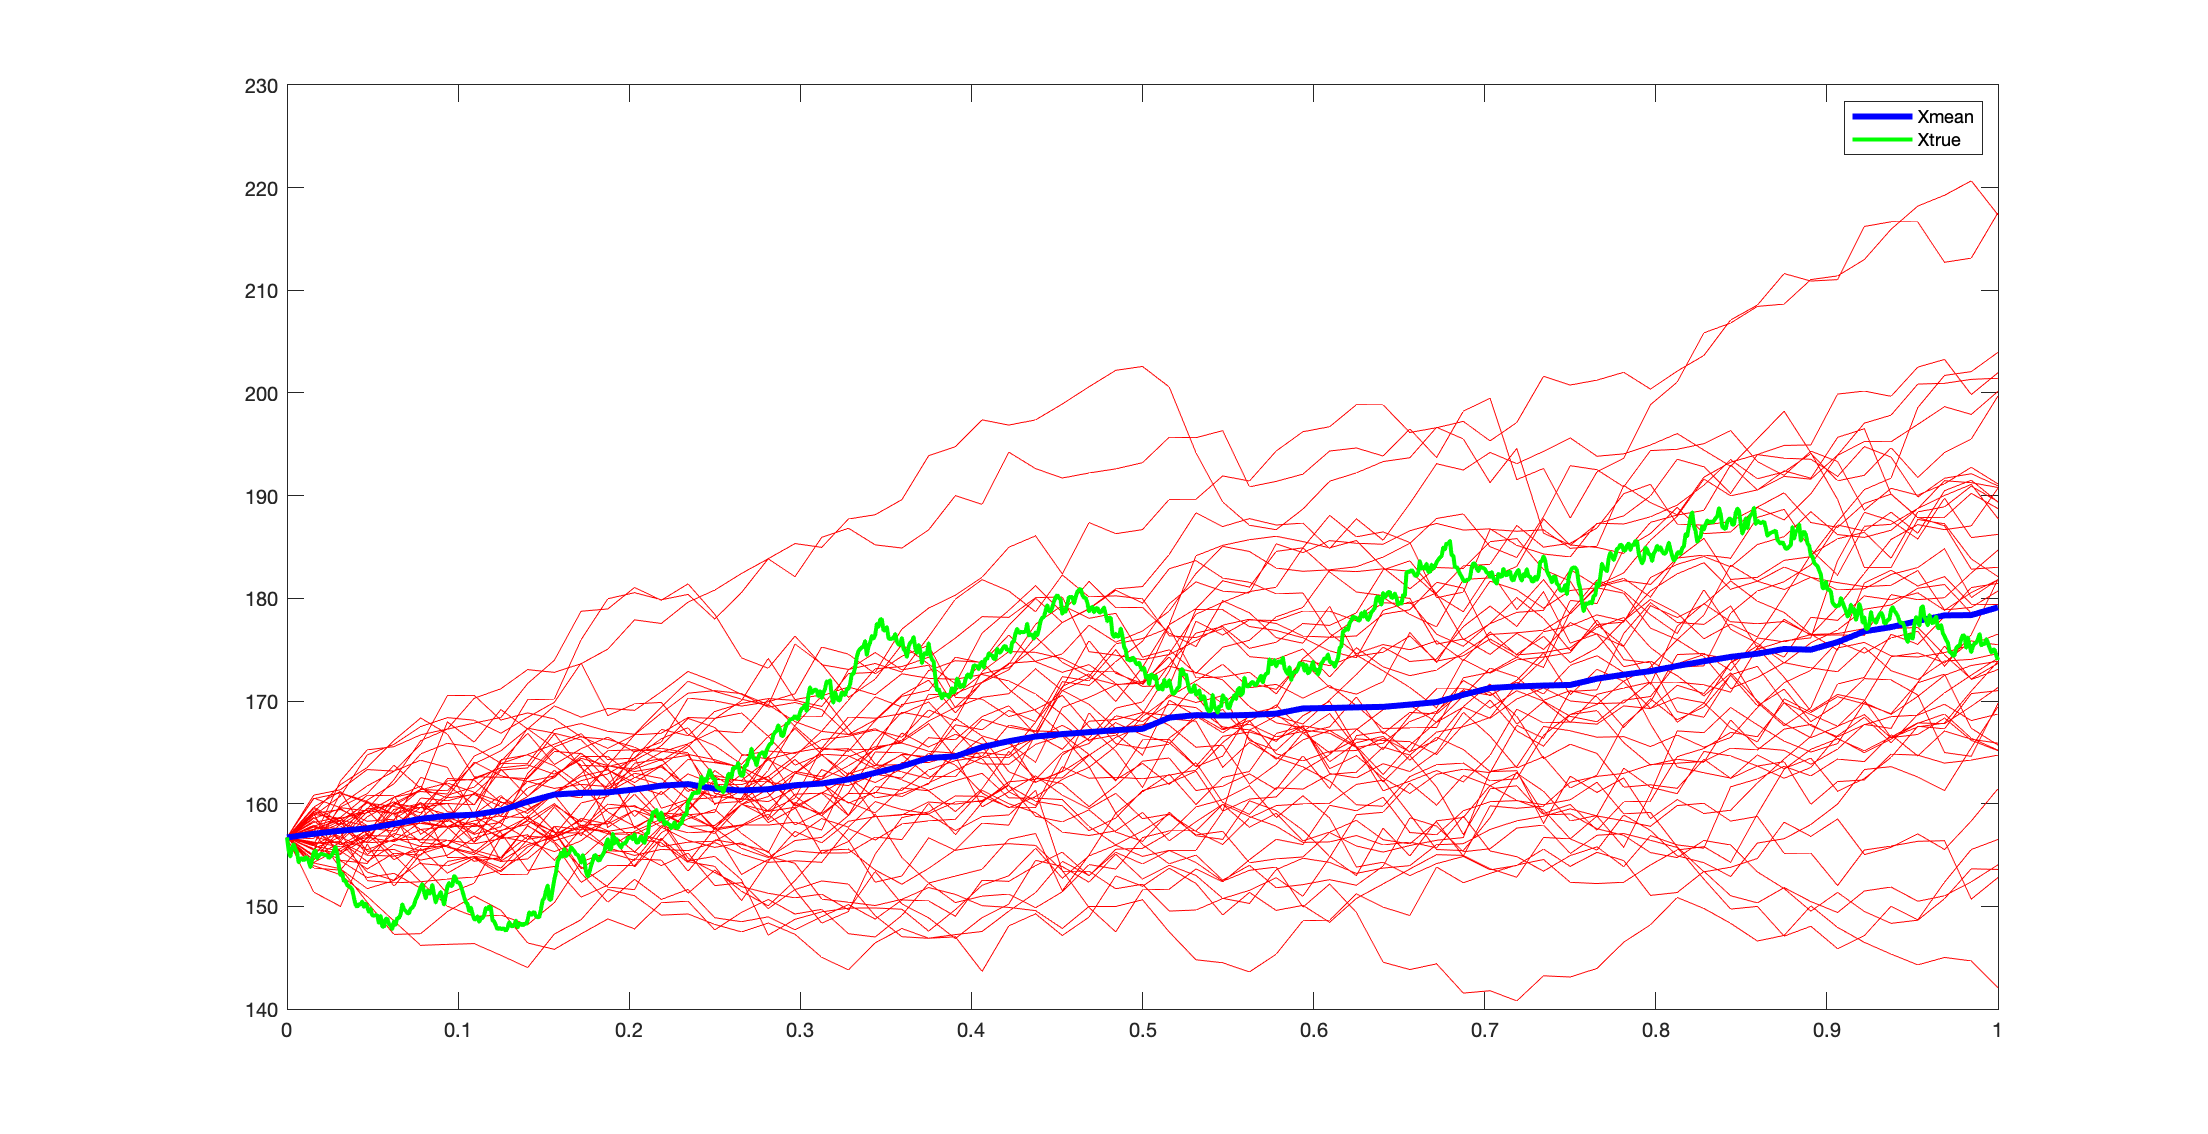
\includegraphics[width=0.9\textwidth]{fig/fig4.png}
\caption{\label{fig4}The first 50 paths of EM method equations when $N=2^6$ with their mean and the true solution }
\end{figure}

For different $N$, we have different value of $\varepsilon_{\Delta t}^{str}$(\verb|mean(Xerr)|), as shown in the following table:
\begin{table}[htbp]
\centering
\begin{tabular}{lll}
\hline
$N$ & $\Delta t$ & \verb|mean(Xerr)| \\ \hline
6   & $2^{-6}$   & \verb|0.1378|     \\
7   & $2^{-7}$   & \verb|0.0971|     \\
8   & $2^{-8}$   & \verb|0.0679|     \\
9   & $2^{-9}$   & \verb|0.0481|     \\
10  & $2^{-10}$  & \verb|0.0340|    
\end{tabular}
\end{table}

From eqn(5.4) in \cite{higham._2001} we take the $\log$ both sides on (\ref{emerr}), which is \begin{equation}
    \label{5.4}
    \log \varepsilon_{\Delta t}^{str} \approx \log C+\frac{1}{2} \log \Delta t.
\end{equation}

We could take $\log-\log$ scale to compare $\varepsilon_{\Delta t}^{str}$ with $\frac{1}{2}$ on plot Fig.\ref{fig5} and we can also take the equation \begin{equation}
    \label{qemerr} \varepsilon_{\Delta t}^{str} = \log C+q\log \Delta t
\end{equation}
with some $q$. A least square fit for $\log C$ and $q$ is shown in the last part in Listing.\ref{lst4}. In this equation, we have \verb|q=0.5052| and \verb|resid =0.0071|, which is consistent with the real order $\frac{1}{2}$.

\begin{figure}[htbp]
\centering
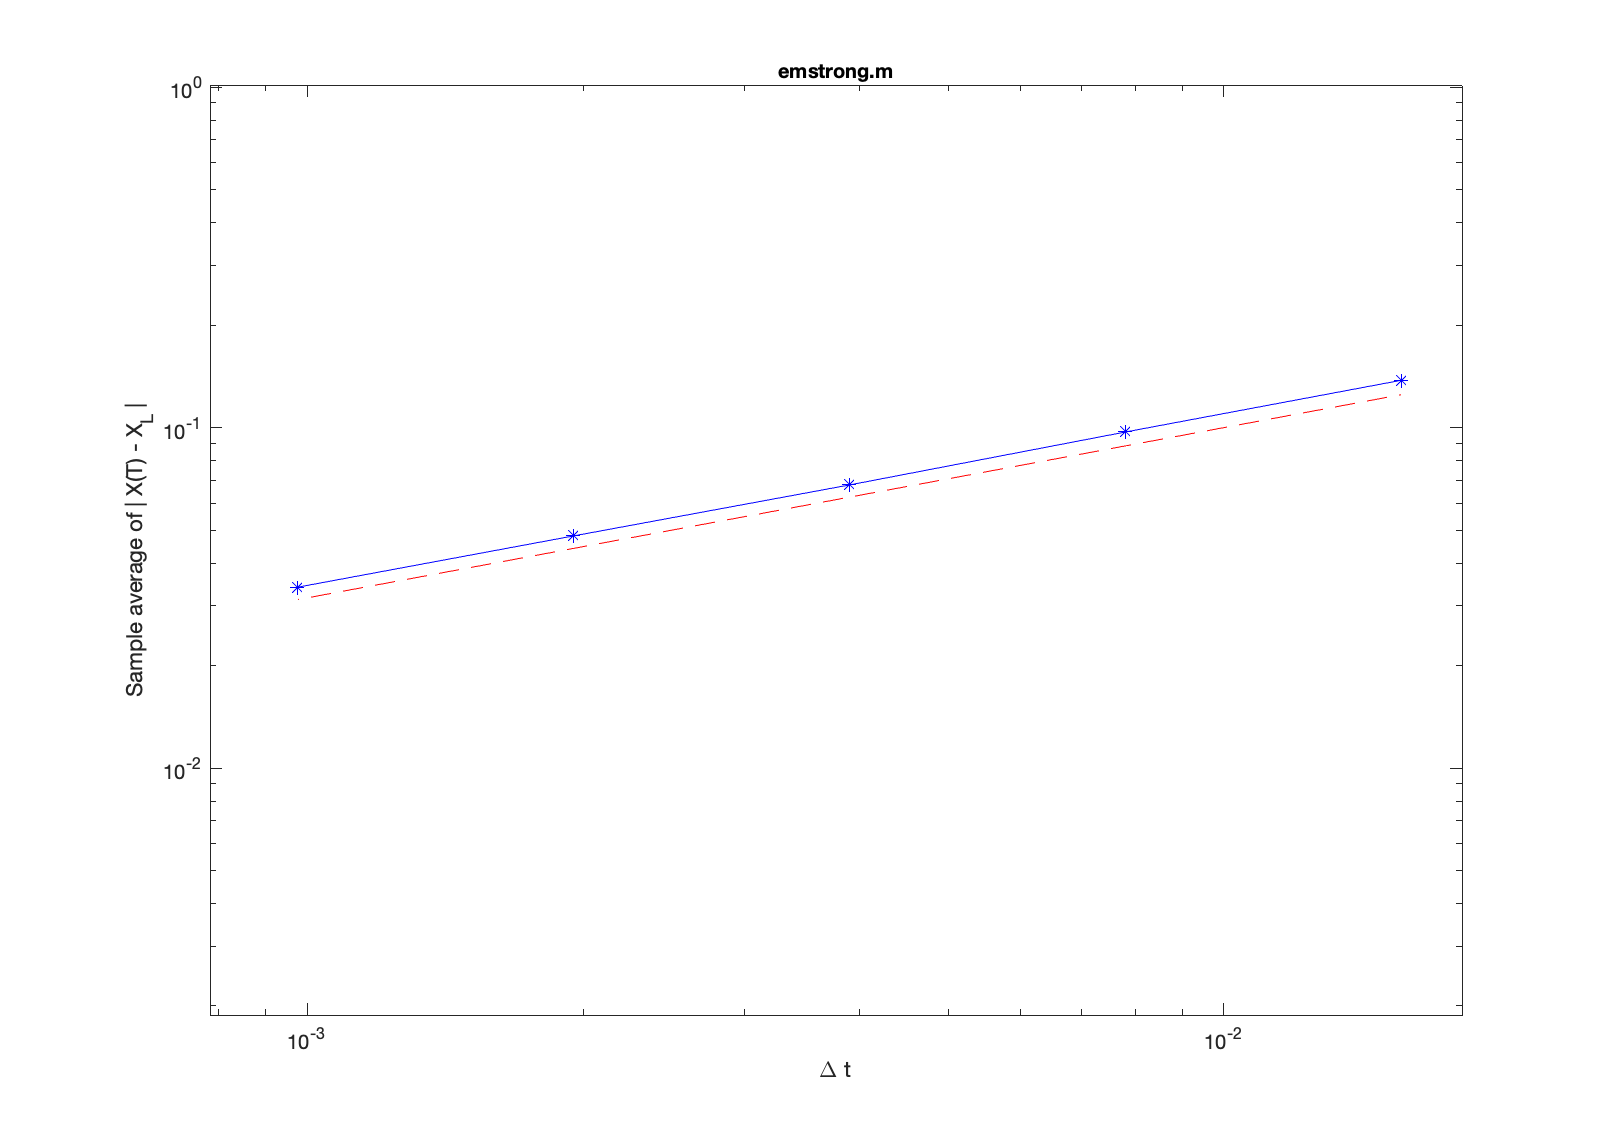
\includegraphics[width=0.7\textwidth]{fig/fig5.png}
\caption{\label{fig5} Comparing the order of error (blue asterisks) with 0.5 (the red line) of strong convergence  }
\end{figure}

When we use MATLAB to calculate $\varepsilon_{\Delta t}^{str}$, there are some types of machine error that may cause bias in our results, they are \cite{higham._2001}: \textit{Sampling error, Random number bias} and \textit{Rounding error.} But in \cite{Saito}, it shows that with the interval $\Delta t$ decreases, the inference of random number bias could be less and we could neglect it when $\Delta t$
is small enough.\\

Now we talk about weak convergence. Weak Convergence  is formalized by suggesting that a sequence of essentially random or unpredictable events may eventually converge into a behavior that is fundamentally stable and unchanging when examined over a sufficiently large number of items in the sequence. We take the form of weak convergence as (eqn(5.6) in \cite{higham._2001}):
\begin{equation}
    \label{weakem} \varepsilon_{\Delta t}^{weak} :=|\mathbb{E}X_{true}(T)-\mathbb{E}X(T)|
\end{equation}

and in \cite{bayram} we know that the order of such weak convergence is 1, which means\begin{equation}
    \label{weakem2} \varepsilon_{\Delta t}^{weak} \le C\Delta t
\end{equation}
for some $C$ (not related to any $t\in [0,T]$) and sufficiently small $\Delta t$. We test it in our equation. The test program in Matlab is displayed in Listing\ref{lst5} (see in \verb|weakcon_em.m|). We set $\mathbb{E}X_{true}(T)=e^{\mu T}$ as the expectation of the true solution and we set 50,000 discrete paths for $N=2^6,2^7,2^8,2^9,2^{10}$ and then we take the mean of those values to obtain $\mathbb{E}X(T)$. Like \verb|strongcon_em.m|, we also use plot to compare $\varepsilon_{\Delta t}^{weak}$ with $1$ and calculate $q$ under a least squares power law. 
\lstinputlisting[caption = {Weak convergence comparing with real order 1}, captionpos=b, label={lst5}]{matlab/weakcon_em.m}
\begin{figure}[htbp]
\centering
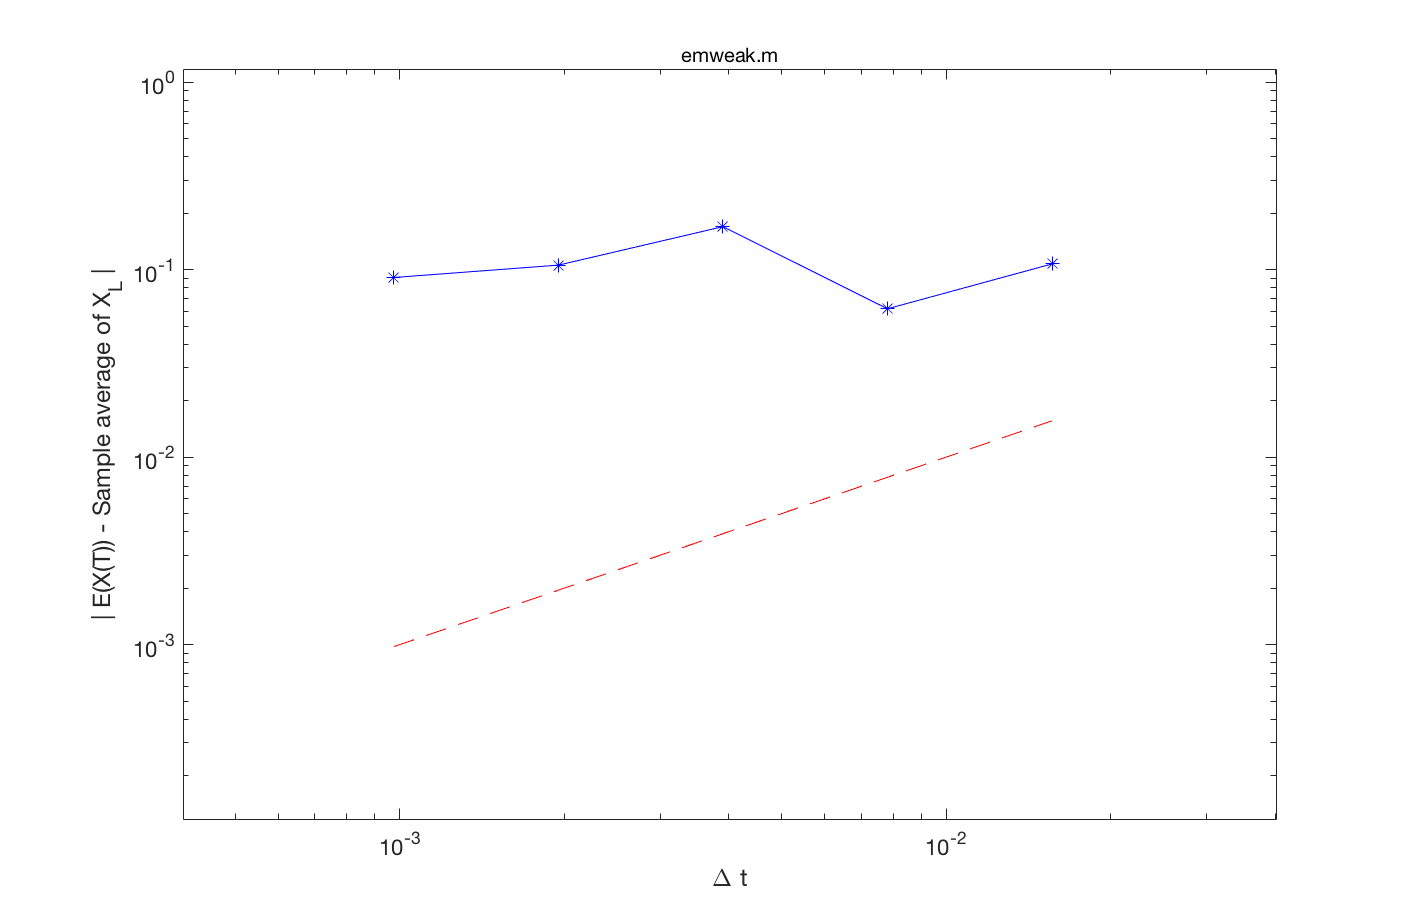
\includegraphics[width=0.7\textwidth]{fig/fig6.png}
\caption{\label{fig6} Comparing the order of error (blue asterisks) with 1 (the red line) of weak convergence  }
\end{figure}

However, when we apply coefficients of $\mu=0.1244$ and $\sigma=0.1038$, we observe that the resulting values of \verb|q=-0.0293| and \verb|resid=0.7224| are far from the expected outcome 1. In contrast, when we use the coefficients $\mu=2$, $\sigma=0.1$, and $X_0=1$ (as in Listing 7 of \cite{higham._2001}), we obtain \verb|q=1.0931| and \verb|resid=0.0985|. We speculate that the reason for this deviation is the high-order decimals in our coefficients, which can introduce round and machine errors that interfere with the true result, especially in the calculation of $\mathbb{E}X_{true}(T)=e^{\mu T}$.

To investigate the impact of the aforementioned issues, we replace $\sqrt{\Delta t}N(0,1)$ with $\sqrt{\Delta t}\text{ sgn}(N(0,1))$ (sign function) and perform the same calculation. We implement this change in \verb|weakcon_em.m| by replacing \lstinline{Winc = sqrt(Dt)*randn(M,1);} with \lstinline{Winc = sqrt(Dt)*sign(randn(M,1));}. With the coefficients set to $\mu=2$, $\sigma=0.1$, and $X_0=1$, the resulting value of \verb|q| is \verb|1.1266|, and \verb|resif| is \verb|0.2253|. This result approximates the expected order of 1. The plot of this result is shown in Fig.\ref{fig7}.


\begin{figure}[htbp]
\centering
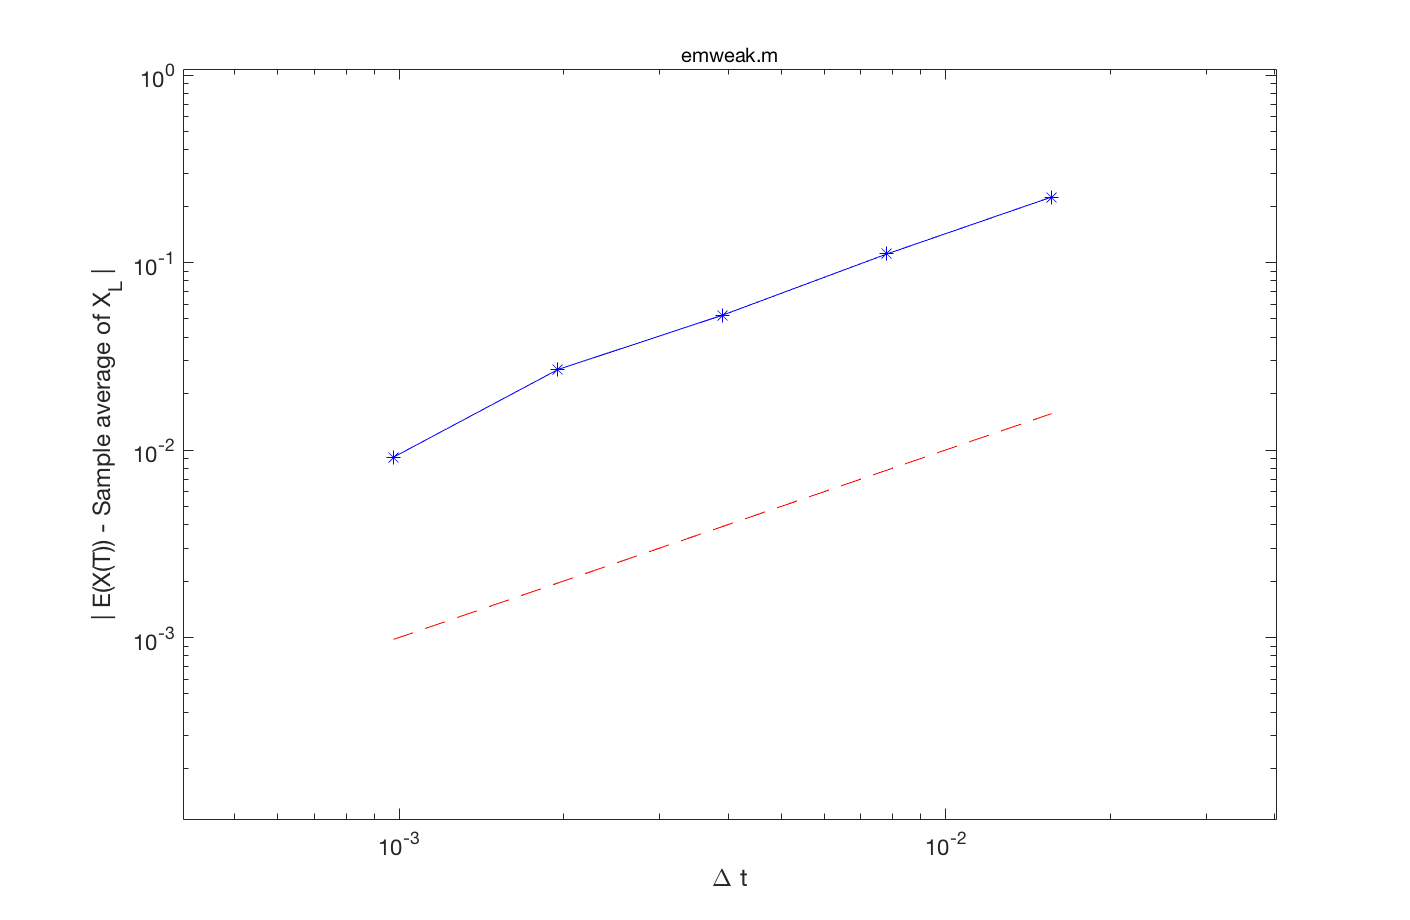
\includegraphics[width=0.7\textwidth]{fig/fig7.png}
\caption{\label{fig7} Replacing   $\sqrt{\Delta t}N(0,1)$ with $\sqrt{\Delta t}\text{ sgn}(N(0,1))$ }
\end{figure}



\section{Milstein Method}
Another method for solving a SDE in numerical method is Milstein method, which is developed by Grigori N. Milstein who first published it in 1974. It is a higher order solution, which we truncate the stochastic Taylor series after second-order terms\cite{bayram} (extract $\mathbb{R}$ in eqn(eq19)). In numerical method form, we write it as: \begin{align}
    X_j =& X_{j-1}+\Delta f(X_{j-1})+g(X_{j-1})\Delta W(t_j)\\
    &+\frac{1}{2}g(X_{j-1})g'(X_{j-1})(\Delta W(X_{j})^2 -\Delta t) ,\quad j=1,2,\dots,n\label{milsteineq}
\end{align}

We apply this method in the SDE (\ref{B-S}), which is $$
dX = \mu X\, dt+ \sigma X\, dW_t.
$$
The Milstein Method in this equation would be written as\begin{equation}
\label{milstein1}
    X(t_{i+1})= X(t_i) + \mu X(t_i) \Delta W(X_i) +\sigma X(t_i)\Delta W(X_i)+\frac{1}{2}\sigma^2 X(t_i) ((\Delta W(X_i))^2-\Delta t)
\end{equation}
Now we apply this method in MATLAB. The first method is that replace \lstinline{Xtemp = Xtemp + Dt*mu*Xtemp + sigma*Xtemp*Winc;} with \lstinline{Xtemp = Xtemp + mu*Xtemp*Dt + sigma*Xtemp.*Winc+ 0.5*sigma^2*Xtemp.*(Winc.^2 - Dt);} in Listing \ref{lst4}, \verb|strongcon_em.m|. We draw the first 50 paths when $N=2^6$ in Fig.\ref{fig8}.
\begin{figure}[htbp]
\centering
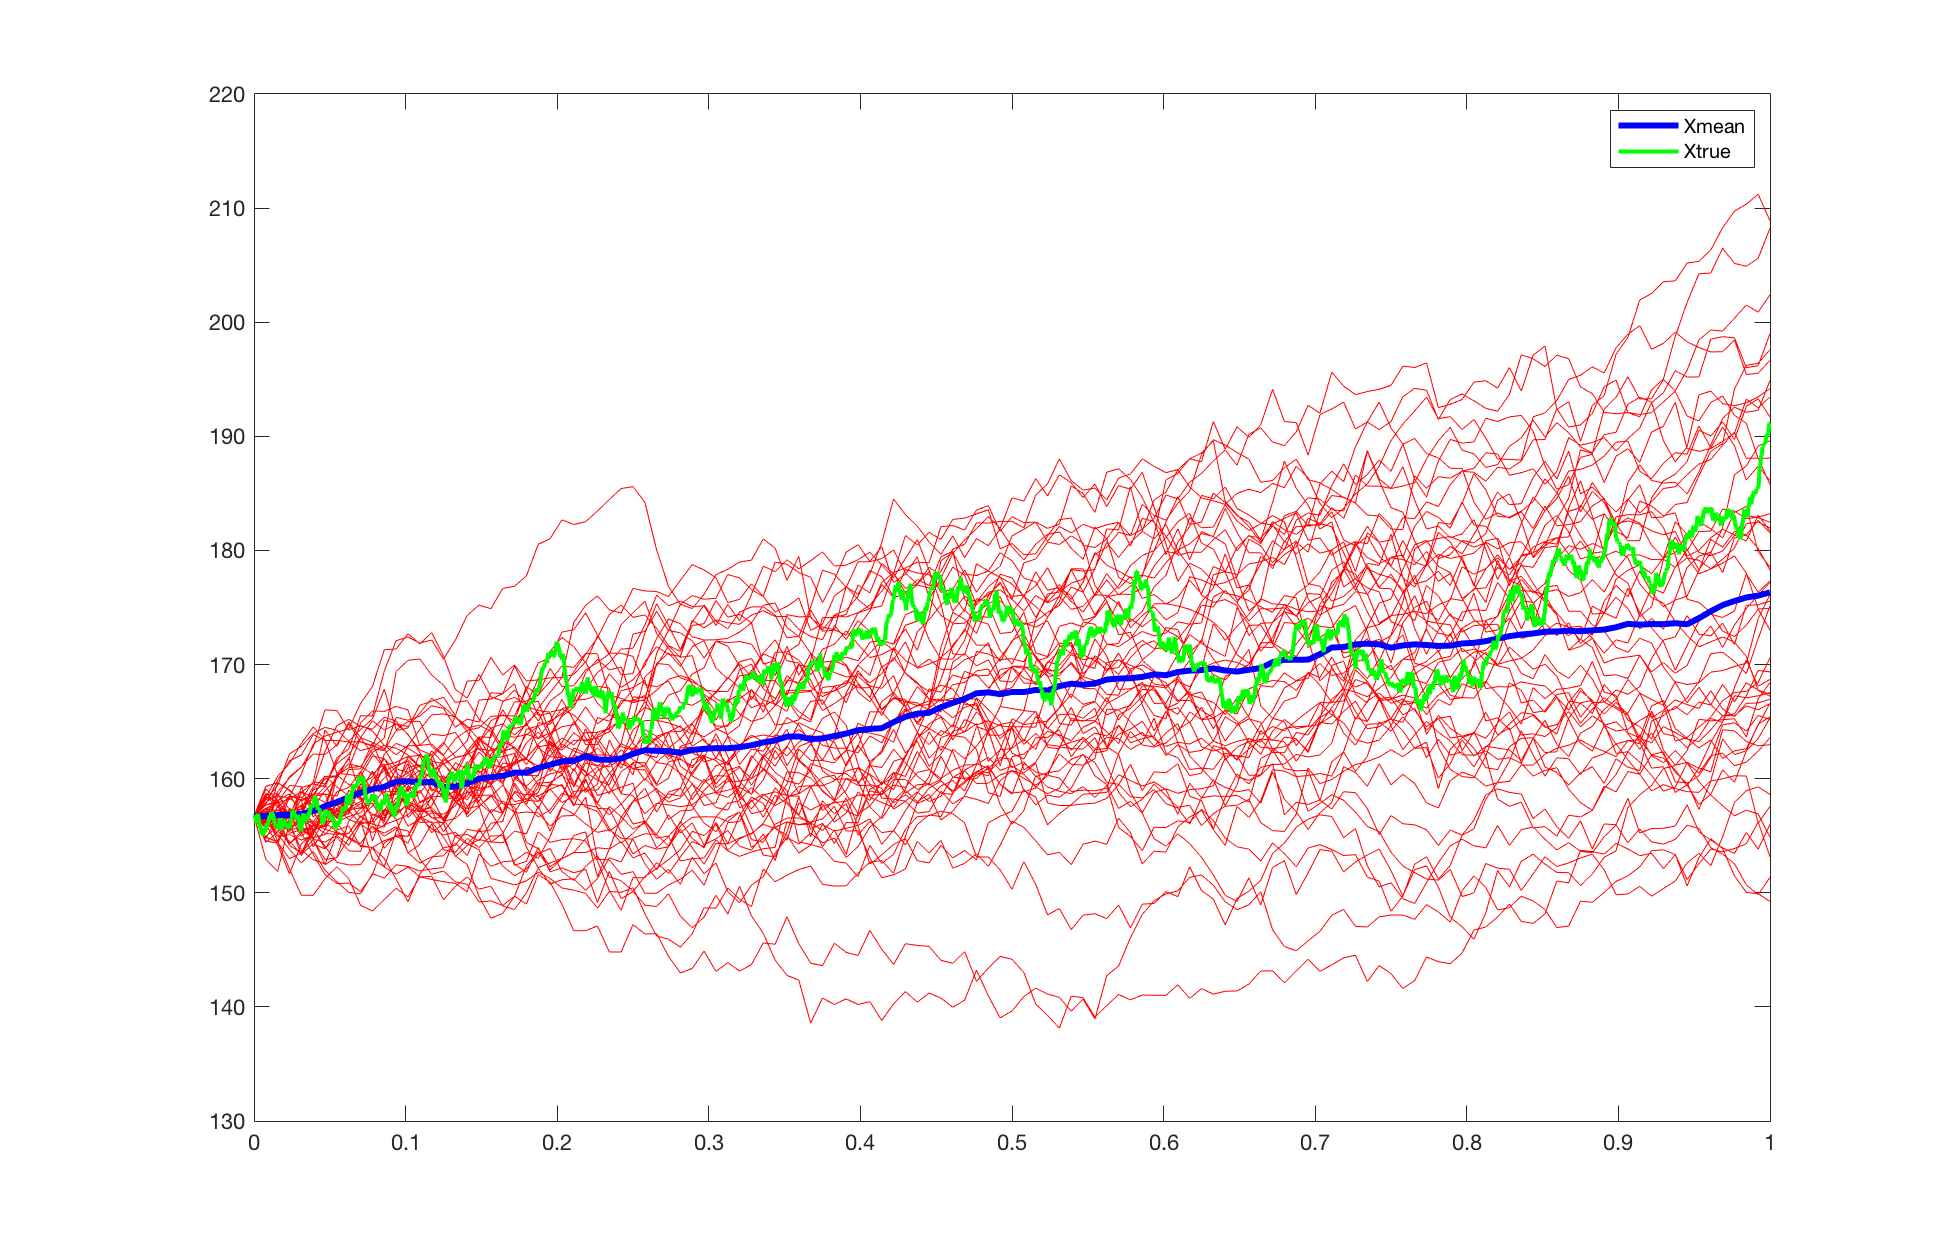
\includegraphics[width=0.9\textwidth]{fig/fig8.png}
\caption{\label{fig8}The first 50 paths of Milstein method equations when $N=2^6$ with their mean and the true solution }
\end{figure}
And then we compare our order $q$ with real order 1. The result shows that \verb|q=0.9999| with \verb|resid=5.1923e-04| , which almost perfectly fit the expect result 1.

\begin{figure}[htbp]
\centering
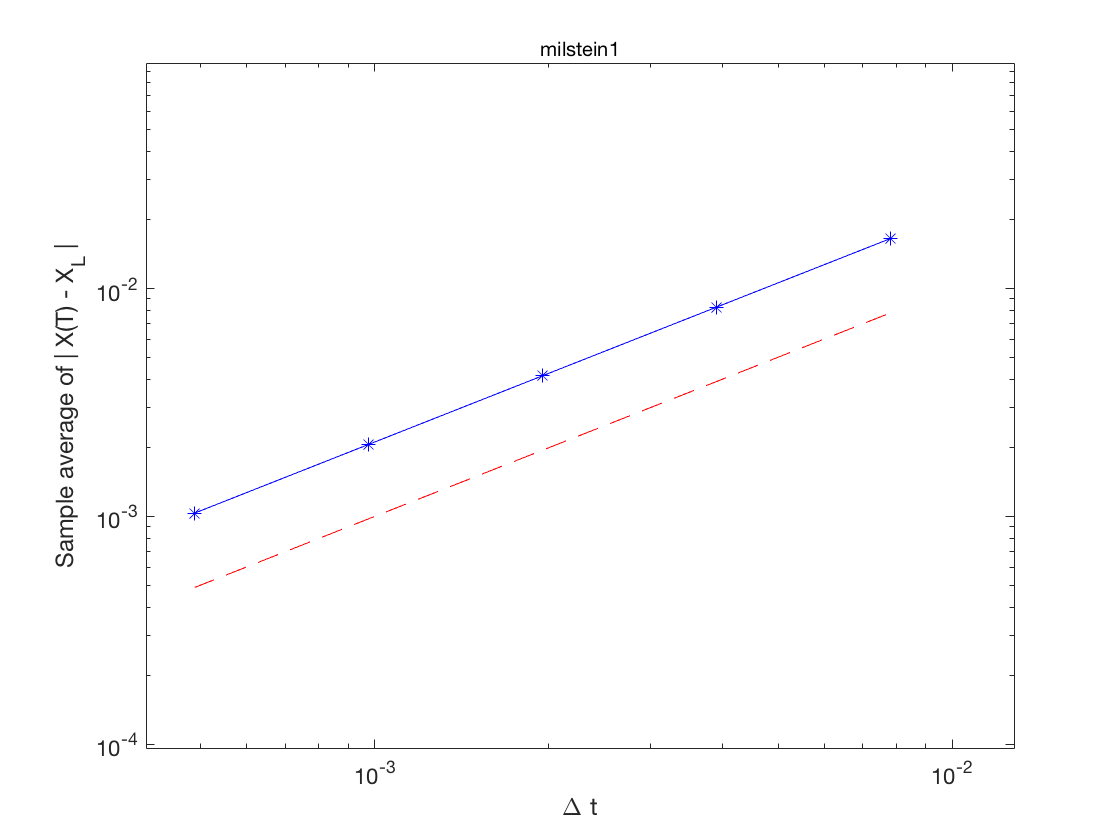
\includegraphics[width=0.7\textwidth]{fig/fig9.png}
\caption{\label{fig9} Comparing the order of error (blue asterisks) with 1 (the red line) of strong convergence (Milstein method)  }
\end{figure}

Another approach to testing the order of strong convergence and calculating errors is to take the smallest interval results (when $N=2^{11}$) as the "true solution". This method can be useful when the real solution of the SDE cannot be obtained, as is often the case with certain SDEs that involve constant parameters, such as $dX(t) = rX(t)(K-X(t))dt+\beta X(t)dW(t)$, where $r, K$, and $\beta$ are constants. And in Listing 8 of \cite{higham._2001}, the author develop the method of calculating different paths- rather than using command \verb|for| to calculate single paths, we set up \verb|dW| as an \verb|M*N| array to compute \verb|n| paths at the same time. The code could be seen in Listing \ref{lst6}, \verb|mlstein.m|. Under this algorithm, \verb|q=1.0246| with \verb|resid = 0.0135|

\lstinputlisting[caption = {Ploting paths (Fig.\ref{fig8}) and comparing with real order 1 in Milstein method}, captionpos=b, label={lst6}]{matlab/milstein.m}

\begin{figure}[htbp]
\centering
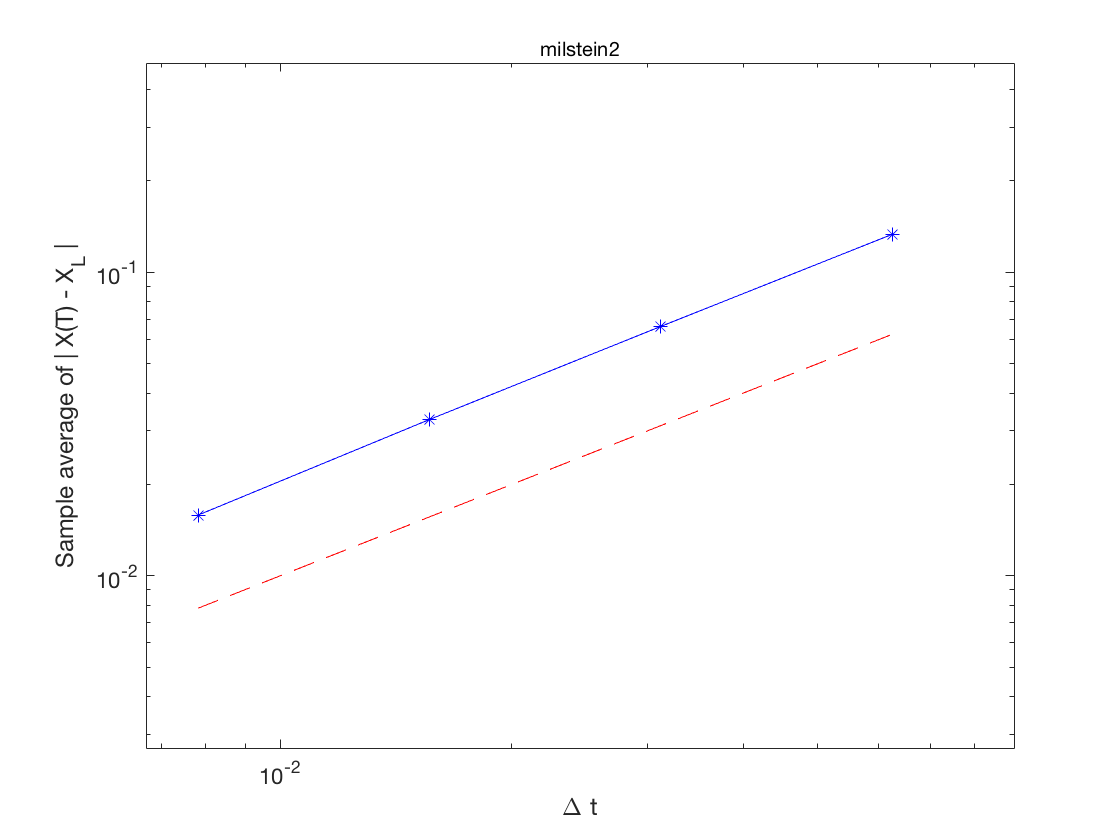
\includegraphics[width=0.7\textwidth]{fig/fig10.png}
\caption{\label{fig10} Comparing the order of error (blue asterisks) with 1 (the red line) of strong convergence (Milstein method) in Listing \ref{lst6} }
\end{figure}

\section{Linear Stability}
In many cases of applications, the time $t$ could be very large, and we should consider the stability of such SDEs. We first consider the simplest ODE \cite{Kloeden}:$$
\frac{dX}{dt}=\lambda X
$$
where $\lambda=\alpha+i\beta\in \C$ is a constant, the solution of this ODE is\begin{equation}
    X(t)=e^{\lambda} t X_0
\end{equation}
We conclude that $|z(t)|=|z_0e^{\lambda t}|\to 0$ if and only if $\alpha=\text{Re}(\lambda)<0$. And in the case $X\equiv 0$ we call it \textbf{asymptotically stable.}

Now we come back to SDE, we consider two measures of stability: mean-square and asympototic. (\cite{higham._2001}, P541). We assume that $X_0\ne 0$ with probability 1, if eqn (\ref{B-S}) satisfy :\begin{equation}
    \label{mscon} \lim_{t\to \infty} \mathbb{E}X(t)^2 = 0\Leftrightarrow \text{Re}(\mu)+\frac{1}{2}|\sigma|^2 <0,
\end{equation}
\begin{equation}
    \label{asycon} \lim_{t\to \infty}|X(t)| = 0\text{, with probability 1}\Leftrightarrow \text{Re}\left(\mu-\frac{1}{2}|\sigma|^2\right)<0,
\end{equation}
where $\mu,\sigma\in \C$, we refer to the left-hand side of (\ref{mscon}) as \textbf{mean-square stability} and (\ref{asycon}) as \textbf{asymptotic stability}. It can be deduced that if an SDE is mean-square stable, then it is also asymptotically stable. However, if an SDE is asymptotically stable, it may not necessarily be mean-square stable.

If we have chosen certain parameters $\mu$ and $\sigma$, we then discuss how the interval $\Delta t$ affect the stability of this SDE. In Euler-Murayama method, it is mean-square stable if $\Delta t$ is small enough, It is clear to analyze it since\begin{equation}
    \label{eq7.3} \lim_{j\to \infty}\mathbb{E}(X(t_j))^2=0\Leftrightarrow |1+\Delta t\mu|^2+\Delta t |\sigma|^2<1
\end{equation}

For asymptotic stability, we consider the strong law of large numbers and the law of the iterated logarithm, and the condition can be written as:\begin{equation}
\label{eq7.4} \lim_{j\to \infty} |X(t_j)|=0 \text{,with probability 1}\Leftrightarrow \mathbb{E}\log|1+\Delta t \mu +\sqrt{\Delta t}\mu N(0,1)|<0.
\end{equation}

We attempted to test both categories of stability in MATLAB using the code provided in \cite{higham._2001} (Listing 9). In the paper, the author tested two cases: $(\mu,\sigma^2)=(-3,3)$ and $(\mu,\sigma^2)=(1/2,6)$ with slopes of $-1$ and $12$, respectively. The author concluded that the former case falls in the "ms" region and the latter falls in the "as" region. These two regions are divided by the line $y=-2x$. We can see it in Fig.\ref{fig11}. We could find that from the figure, EM mean-square stability require the slope should be less than -2 and the lower value of slope, the less liability of $\Delta t$ requires.

\begin{figure}[htbp]
\centering
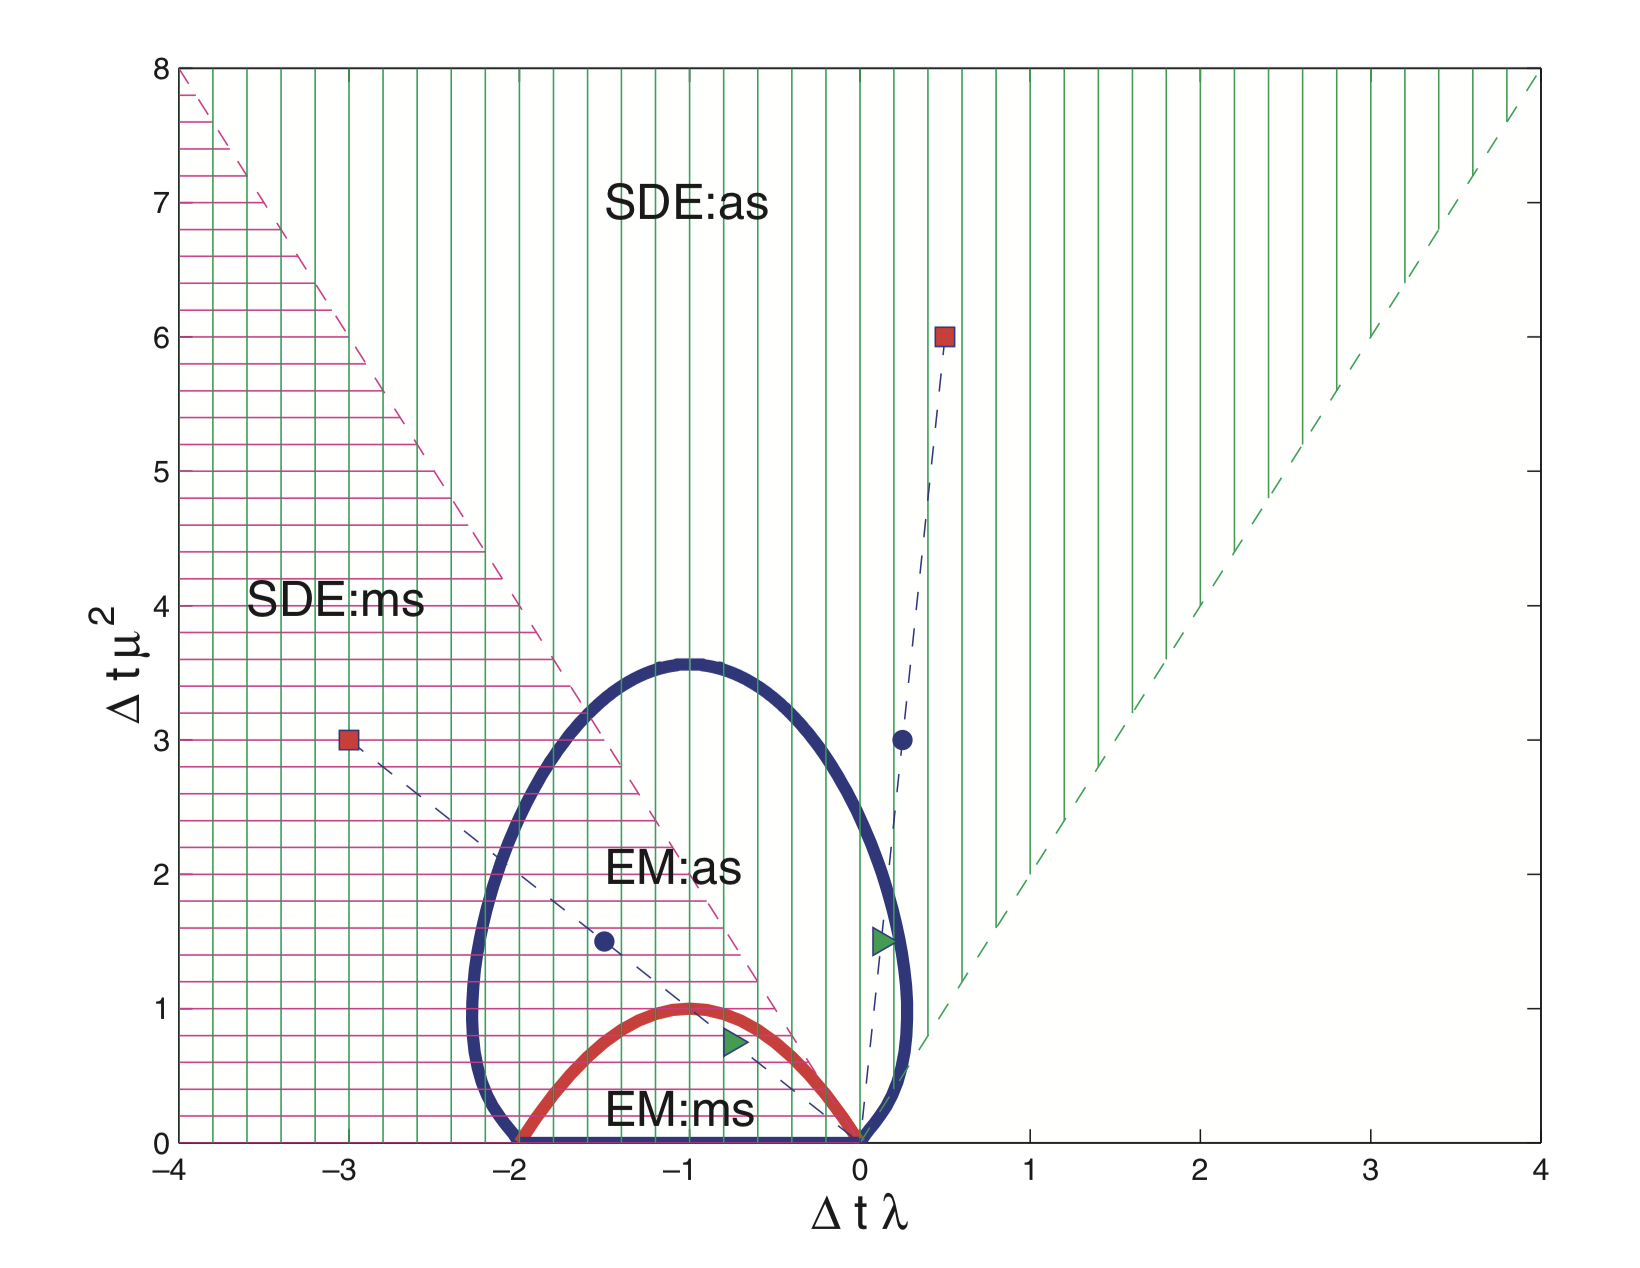
\includegraphics[width=0.6\textwidth]{fig/fig11.png}
\caption{\label{fig11} Mean-square and asymptotic stability regions. (It is from \cite{higham._2001}, Fig.6) }
\end{figure}


Now we try different parameters to test stability. First we try $(\mu,\sigma^2)=(-1,0.5)$ of mean-square stability, which shows that all test points can all fall in 'EM:ms' region in Fig.\ref{fig11} and  $(\mu,\sigma^2)=(0.02,2)$ which shows that all test points can all fall in 'EM:as' region in Fig.\ref{fig12}. As we plot them on Fig.\ref{fig12}, we find that they are all stable.

\begin{figure}[htbp]
\centering
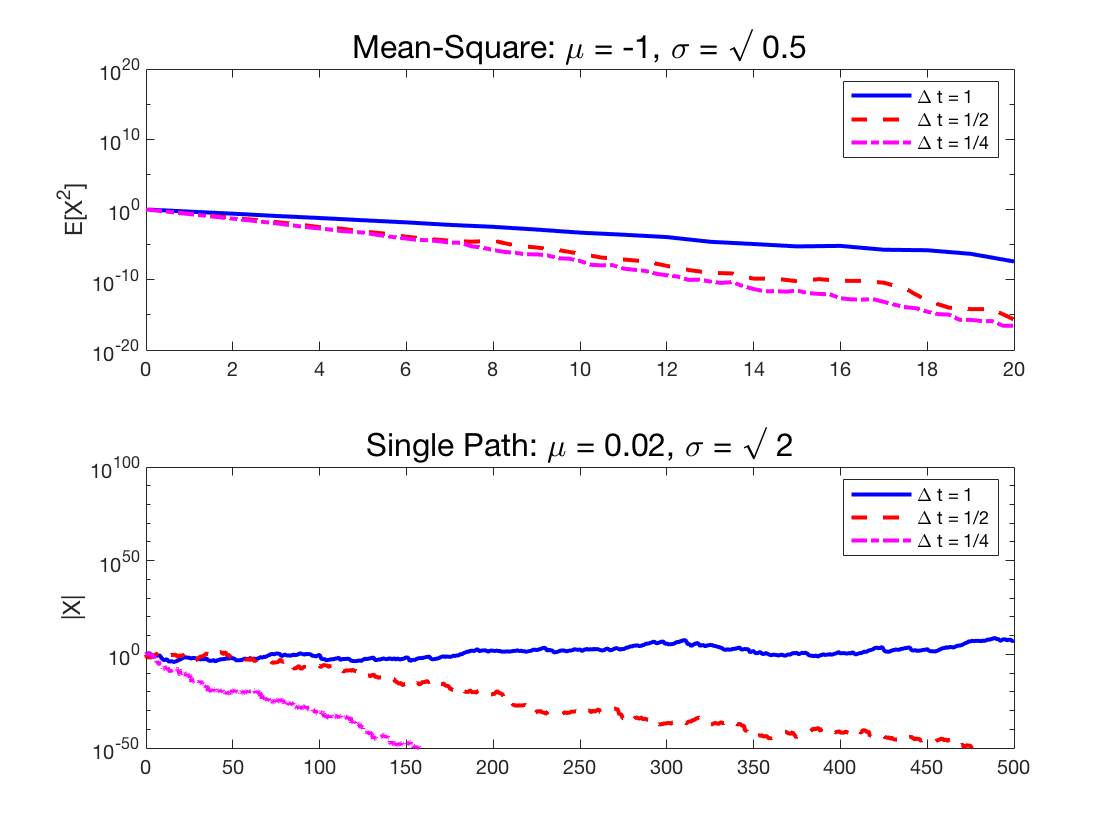
\includegraphics[width=0.6\textwidth]{fig/fig12.png}
\caption{\label{fig12} Mean-sqaure and asympototic tests }
\end{figure}

Now we test stability of our equation (\ref{emeq2}) with coefficient $(\mu,\sigma^2)=(0.1244,0.1038^2)$ and slope $0.0866$. By the result we find that all points falls out of stable regions, whether they are in 'ms' region or 'as' region. We test it in \verb|stability.m|. The result is shown in Fig.\ref{fig13}. It is clear that $E[X^2]$ and $|X|$ all expand to large numbers as $t$ increases. Thus, our equation (\ref{emeq2}) tested before is not stable.

\begin{figure}[htbp]
\centering
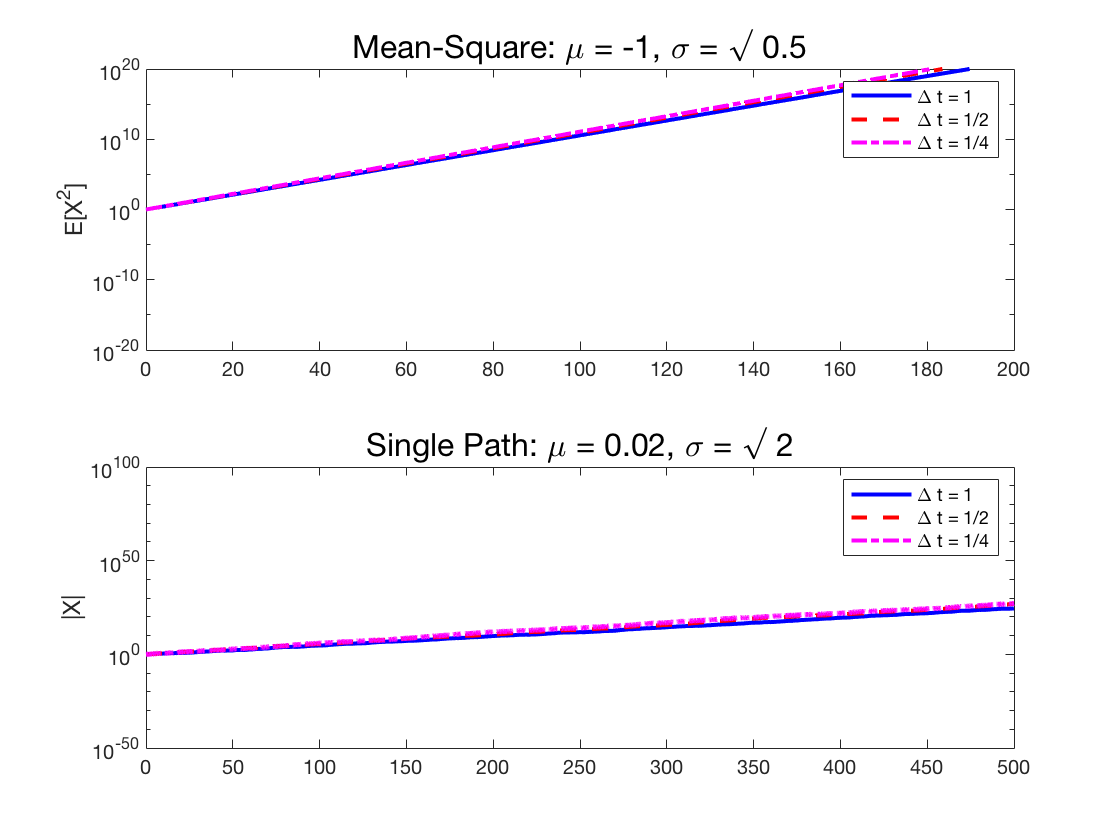
\includegraphics[width=0.6\textwidth]{fig/fig13.png}
\caption{\label{fig13} Mean-sqaure and asympototic tests of eq(\ref{emeq2})}
\end{figure}

\section{Pseudo-random and Quasi-random Numbers}
\subsection{Quasi-random numbers and Box-Muller Method}
As previously discussed, we currently generate our Wiener process in MATLAB using pseudo-random numbers. However, according to \cite{sauer}, the independence of stochastic variables is not a crucial factor in computations. Therefore, we can optimize our algorithm by incorporating quasi-random numbers, which are also known as low-discrepancy numbers due to their low discrepancy as we define discrepency as \cite{kuipers}:\begin{defn}
    Let $x_1,\dots, x_N$ be a finite series of real numbers. We define$$
    D_N=\sup_{0\le\alpha\le \beta\le 1}\left|\frac{\#\{\{x_1,\dots,x_N\}\bigcap [\alpha, \beta)\}}{N}-(\beta-\alpha)\right|
$$
    As the discrepancy of giving sequence $\{x_1,\dots,x_N\}$.
\end{defn}
We remark that in this baby version definition we just use the length of interval $[\alpha, \beta)$ instead of Lebesgue measure. Quasi-random sequences are identically-distributed but not independent. However, they are better at self-avoidance compared to pseudo-random numbers and they can provide Monte Carlo approximations with significantly reduced variance while using the same number of realizations.

When estimating expected values like (\ref{emeq2}) by calculating many realizations, the $m$ increments $\Delta W_1,\dots,\Delta W_m$ of each realization must be independent. To maintain independence along the trajectories, it is essential to use $m$ different low-discrepancy sequences. To produce low-discrepancy numbers, we can apply \textbf{Box-Muller method}. \cite{box-muller}

Let $U_1, U_2$ be independent random variables of uniform distribution on the unit interval $(0,1)$, then we define \begin{equation}
    \label{BMx1} X_1=(-2\log U_1)^{1/2}\cos 2\pi U_2
\end{equation}
\begin{equation}
    \label{BMx2} X_1=(-2\log U_1)^{1/2}\sin 2\pi U_2
\end{equation}
Then we have $(X_1, X_2)$ is a pair of independent random variables and have the same normal distribution $N(0,1)$.

We generate quasi-random number in MATLAB as follow:
\begin{lstlisting}[ caption={Generating quasi-random numbers in MATLAB},captionpos=b,label={lst7}]
U_1 = rand(1,100000);
U_2 = rand(1,100000);
R0 = sqrt(-2*log(U_1));
theta = 2*pi*U_2;
x = R0.*cos(theta);
y = R0.*sin(theta); % generate quasi-random numbers
\end{lstlisting}

In Listing \ref{lst7}, we use quasi-random number vectors \verb|x| and \verb|y|, which are shown in Fig \ref{fig14}. The mean and variance of \verb|x| are \verb|mean = 0.0020| and \verb|var = 1.0008|, respectively. The mean and variance of \verb|y| are \verb|mean = -0.0028| and \verb|var = 0.9989|, respectively. These values indicate that the mean and variance of quasi-random numbers are very close to those of a standard normal distribution.

\begin{figure}[htbp]
\centering
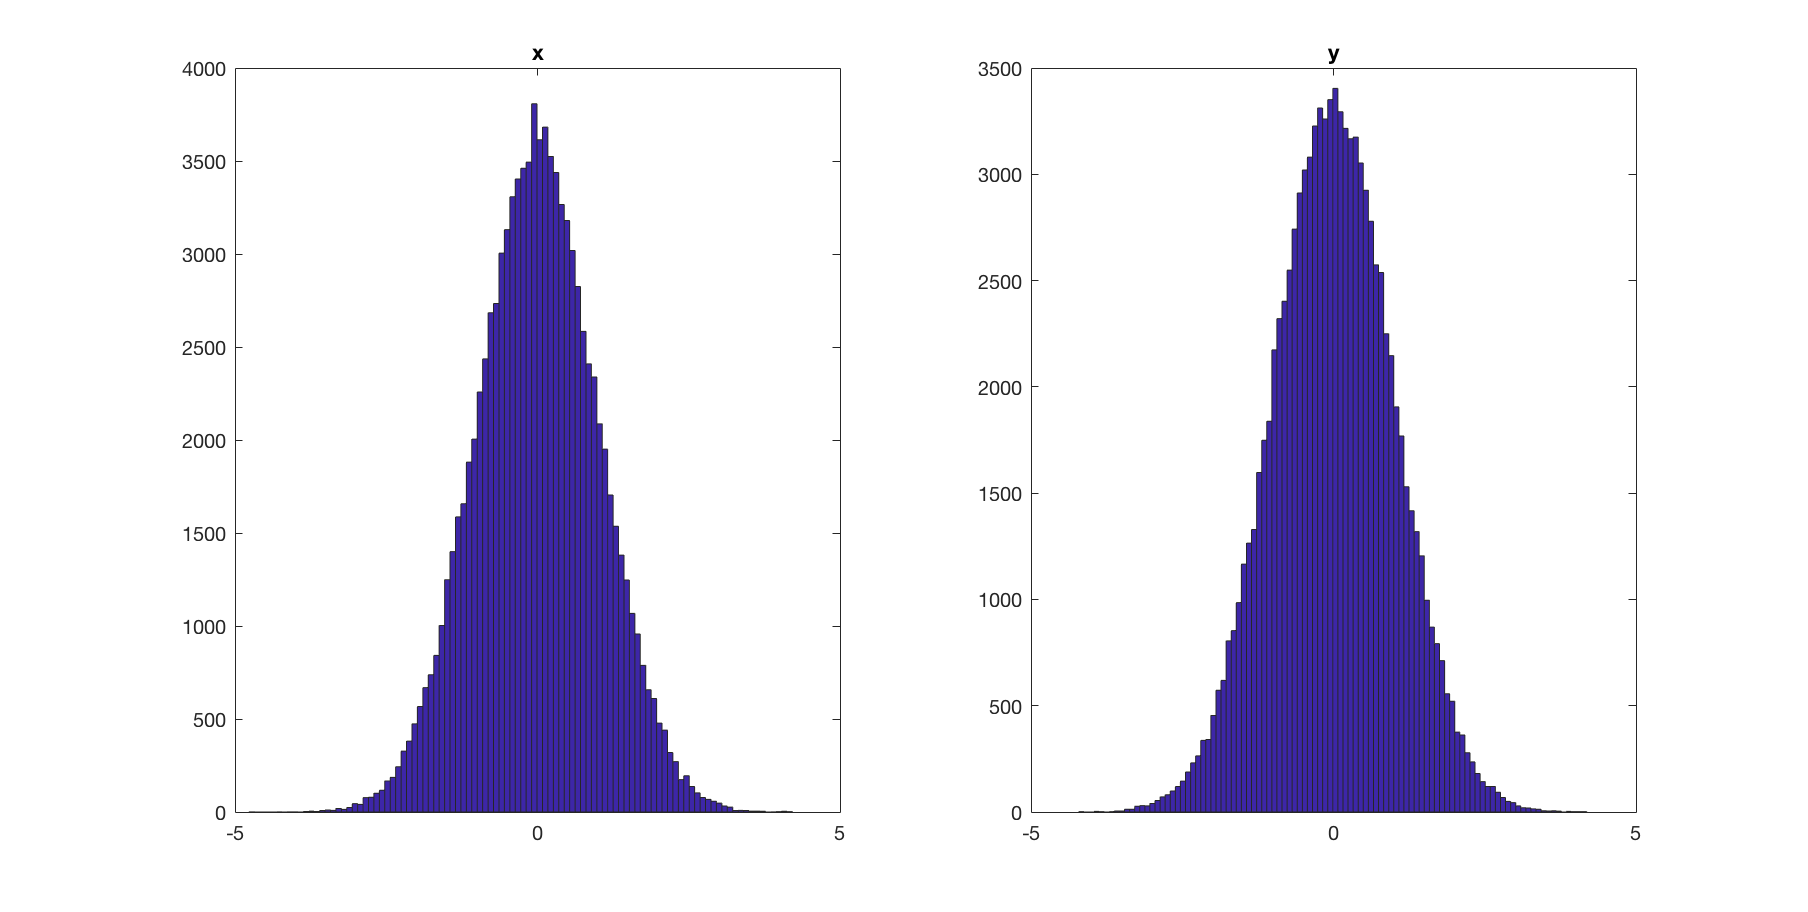
\includegraphics[width=0.8\textwidth]{fig/fig14.png}
\caption{\label{fig14} Histogram of quasi-random number vectors x and y}
\end{figure}

\subsection{European Call Option}
Now we test the differences in MATLAB. However, if we test the previous equation, the true solution (\ref{trueAAPL}) contains random terms which we need to avoid. Thus, we consider the \textbf{European call option} (\cite{bjork}, P98). A European call option contains exercise price $K$, time of maturity $T$ and underlying asset $S$. It is defined as \begin{itemize}
    \item At time T, the holder of the option has the right to purchase one share of the underlying stock from the option underwriter at a price of $K$ dollars.

    \item The holder is under no obligation to exercise this right and purchase the stock. 

    \item The option can only be exercised at the exact time $T$, and not at any other time.
\end{itemize}

We give its contract function as:
\begin{equation}
    \Phi(x) = \max [x-K,0]
\end{equation}

If we consider no arbitrage condition, the present value (details can be looked up in \cite{bjork} P100-108) of the assumption is: 
\begin{equation}
    F(X_0,T) = e^{-rT}\mathbb{E}_{t,s}^Q \{\max [X(T)-K,0]\},
\end{equation}
where $r$ is the risk-free interest rate and the underlying stock price $X(t)$ satisfies the Black-Scholes equation:\begin{equation}
    dX = rX\, dt+\sigma X\, dW_t^Q.
\end{equation}
We denote that $W_u^Q$ is $Q$-dynamics under $Q$ martingale. Then we could get the true solution under time $T$:\begin{equation}
    \label{trueEuro} F(X,T)= XN(d_1)-Ke^{-rT}N(d_2) ,
\end{equation}
where $$
d_1 = \frac{\log(X/K)+(r+\frac{1}{2}\sigma^2)T}{\sigma \sqrt{T}},\quad d_2 = d_1-\sigma \sqrt{T-t}.
$$ and$$
N(d) = \frac{1}{\sqrt{2\pi}}\int_{-\infty}^d e^{-\frac{t^2}{2}}\, dt
$$

We compute it in MATLAB in Listing 8. We set $X(0)=10$, $K=12$, $r=0.05$, $\sigma = 0.5$ and $T=0.5$. 

\begin{lstlisting}[ caption={Computing exact solution of European call option},captionpos=b,label={lst8}]
syms t d
S = sym(10);        % current stock price (spot price)
K = sym(12);         % exercise price (strike price)
sigma = sym(0.50);   % volatility of stock
T = sym(0.5);       % expiry time in years
r = sym(0.05);       % annualized risk-free interest rate

PV_K = K*exp(-r*T);
d1 = (log(S/K) + (r + sigma^2/2)*T)/(sigma*sqrt(T));
d2 = d1 - sigma*sqrt(T);
Nd1 = int(exp(-((t)^2)/2),-Inf,d1)*1/sqrt(2*pi);
Nd2 = int(exp(-((t)^2)/2),-Inf,d2)*1/sqrt(2*pi);
C = Nd1*S - Nd2*PV_K;

Csym = Nd1*S - Nd2*PV_K;
Cvpa = vpa(Csym)

[Call, Put] = blsprice(double(S), double(K), double(r), double(T), double(sigma))
\end{lstlisting}

Or in the last line of Listing \ref{lst8}, we can directly apply the function \lstinline{[Call,Put] = blsprice(Price,Strike,Rate,Time,Volatility)} to get the true solution of the European call option.

\subsection{Test of Pseudo-random numbers and Quasi-random numbers in MATLAB}

Now we test the differences in MATLAB (\verb|quasi.m|), we set $\Delta t$ as $2^{-11},\dots 2^{-5}$:

\lstinputlisting[caption = {Comparsion of errors between pseudo-random and quasi-random numbers}, captionpos=b, label={lst9}]{matlab/quasi.m}

We plot the result in Fig. \ref{fig15} and denote the errors in the Table \ref{tb2}:
\begin{figure}[htbp]
\centering
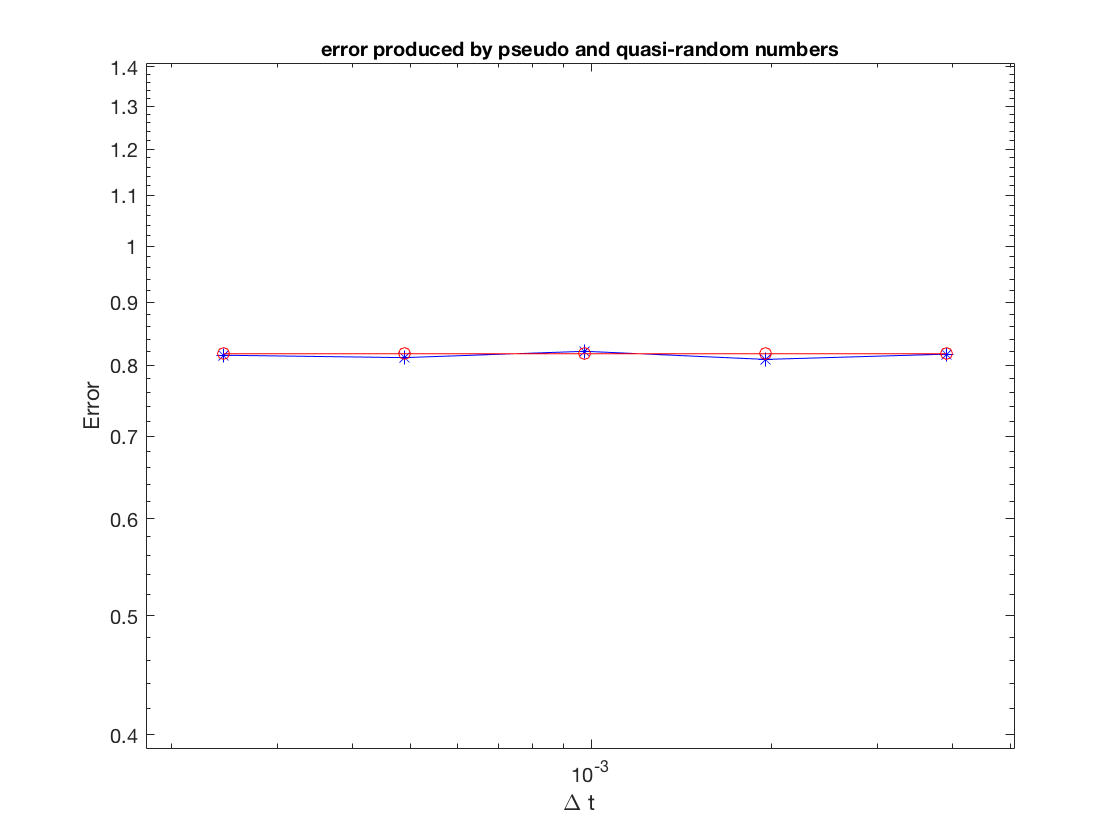
\includegraphics[width=0.6\textwidth]{fig/fig15.png}
\caption{\label{fig15} Histogram of quasi-random number vectors x and y}
\end{figure}


% Please add the following required packages to your document preamble:
% \usepackage{longtable}
% Note: It may be necessary to compile the document several times to get a multi-page table to line up properly
\begin{longtable}[c]{llllll}
\hline
\textbf{Power of (-$\Delta t$)} & \textbf{11} & \textbf{10} & \textbf{9} & \textbf{8} & \textbf{7} \\ \hline
\endfirsthead
%
\endhead
%
pseudo-                       & 0.8150      & 0.8114      & 0.8210     & 0.8087     & 0.8166     \\
quasi-                        & 0.8172      & 0.8172      & 0.8172     & 0.8172     & 0.8172    \\ \hline
\caption{Errors between pseudo- and quasi-random numbers}
\label{tb2}\\
\end{longtable}

However, we failed to obtain the expected result (which is shown in Fig.\ref{fig16} from \cite{sauer}). 

\begin{figure}[htbp]
\centering
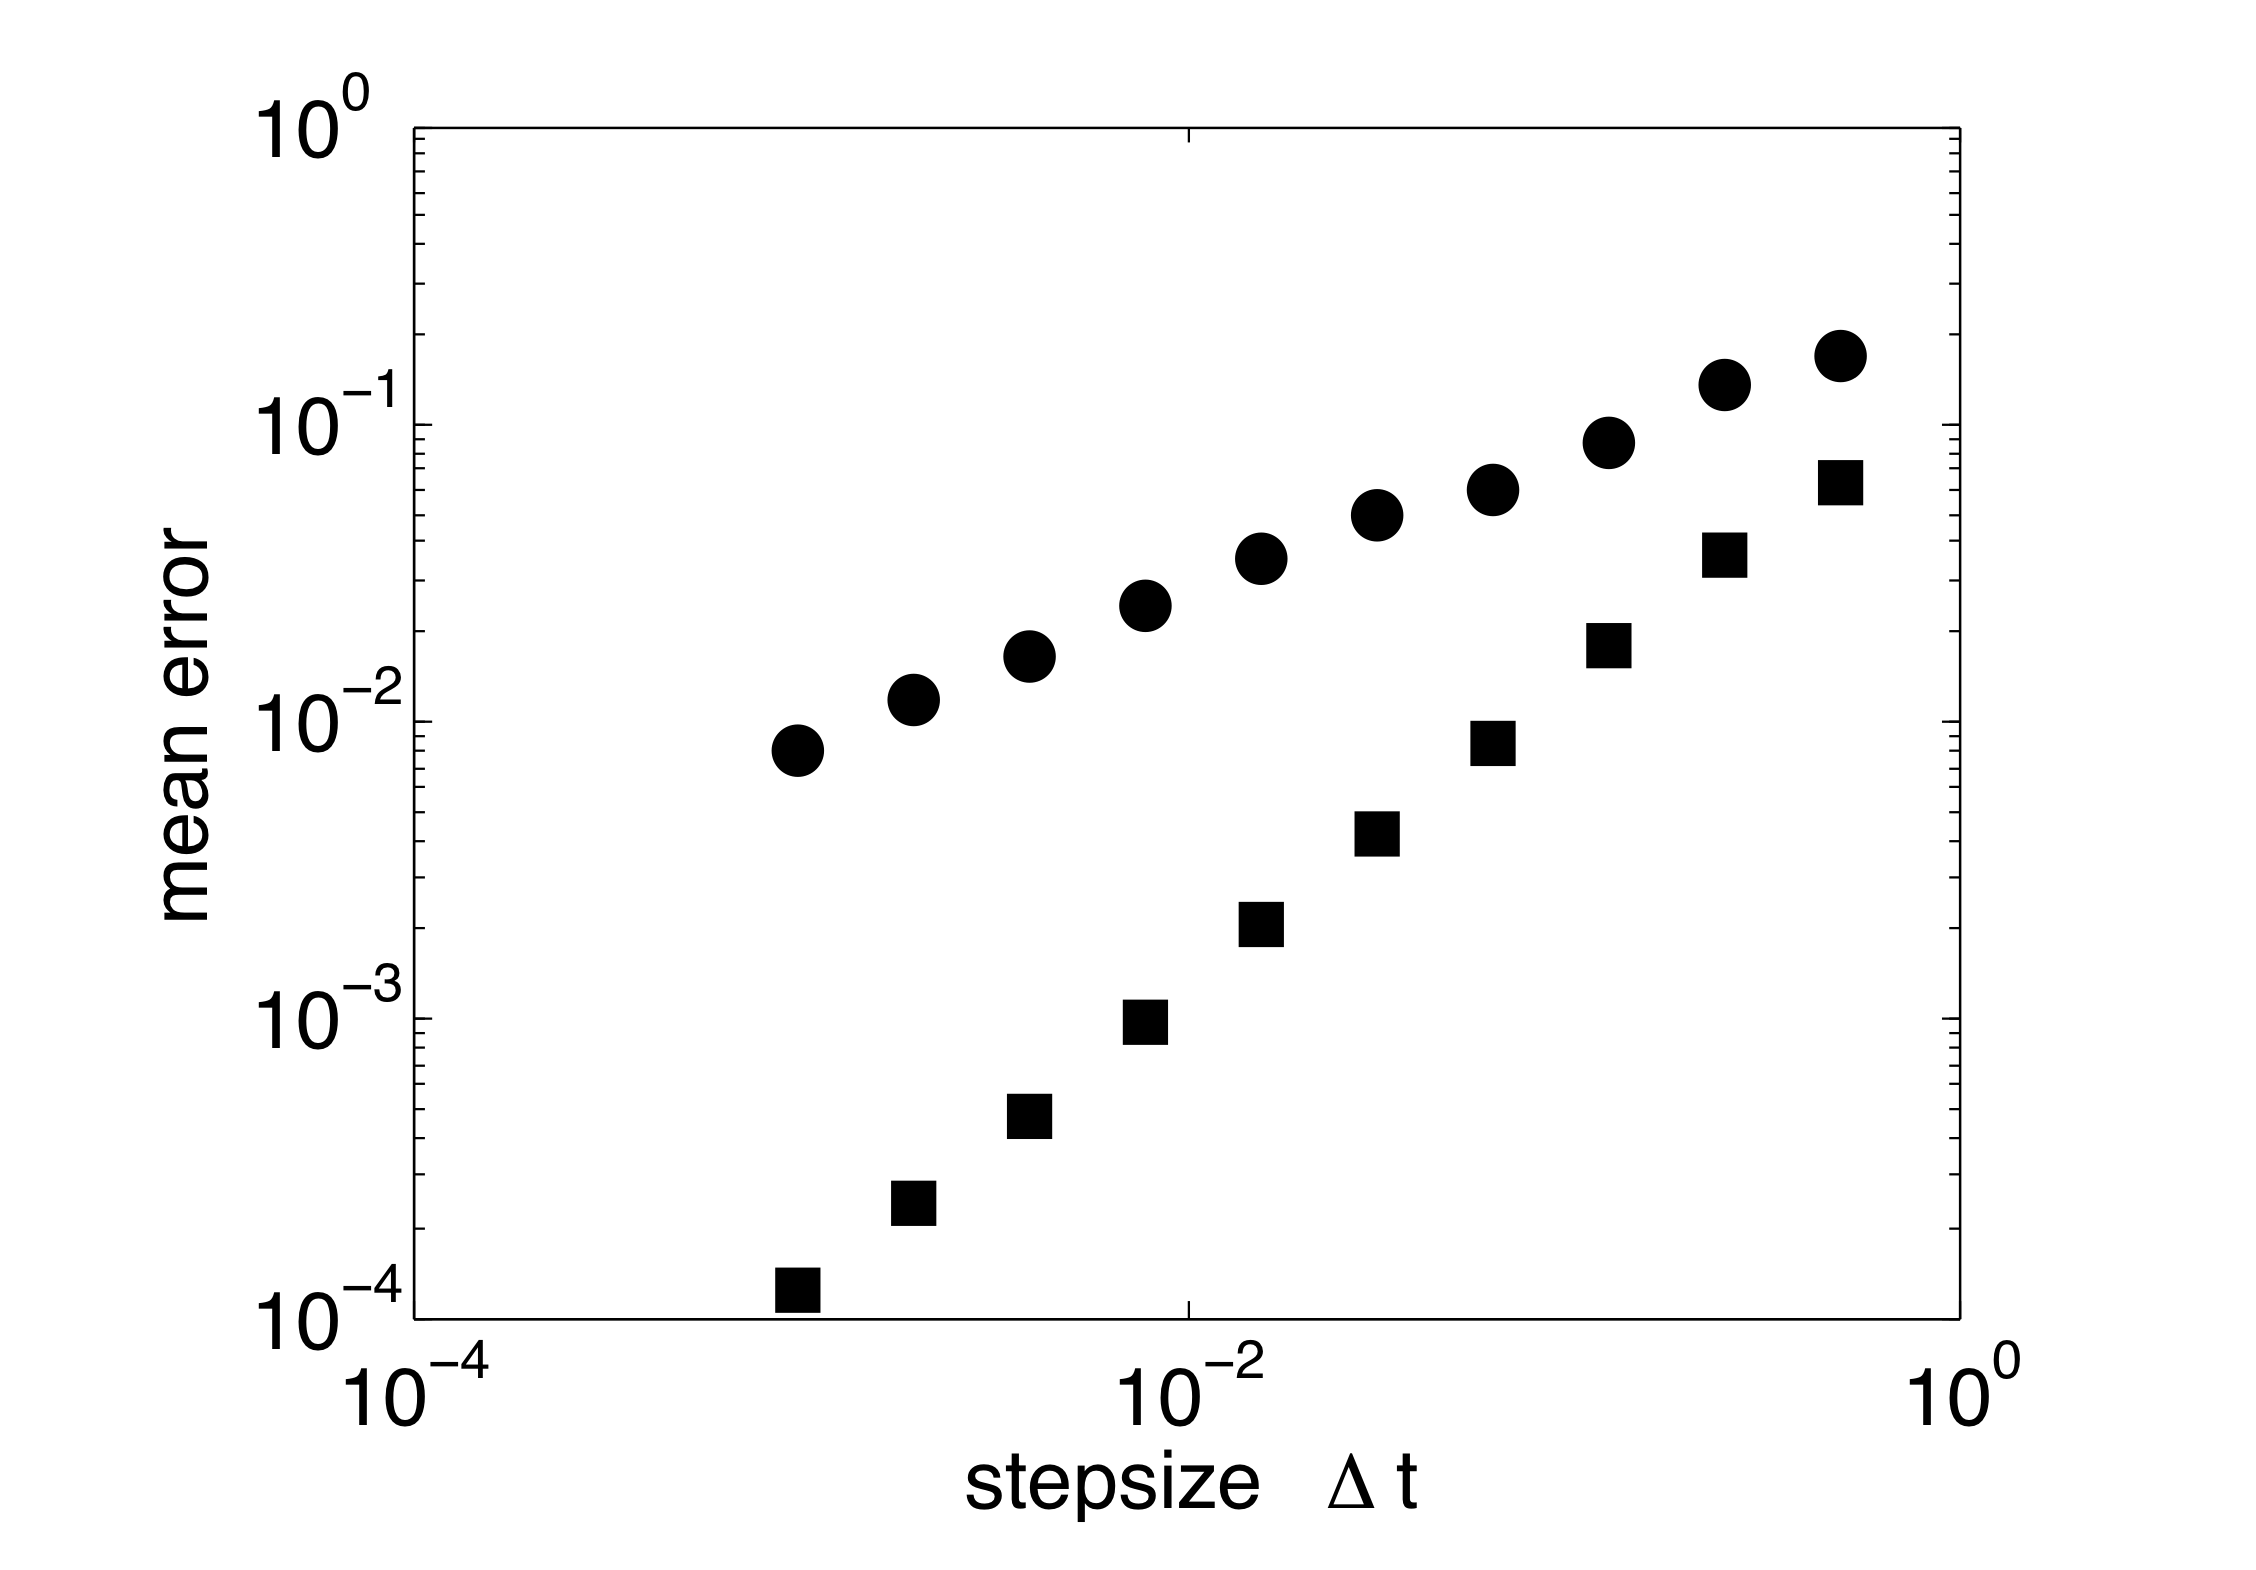
\includegraphics[width=0.6\textwidth]{fig/fig16.png}
\caption{\label{fig16} The expected results (square for quasi- and circle for pseudo-)}
\end{figure}


Despite our best efforts, we encountered difficulties that prevented us from achieving the desired outcome. Potential factors contributing to this failure include machine errors or incorrect generation of random numbers. Following the instructor's recommendation, we have documented these erroneous results in the paper. Moving forward, we are hopeful that with the assistance of an expert in numerical analysis, we can overcome these challenges and find a resolution.

\section{Summary}
\newpage
\printbibliography
\end{document}       